% Options for packages loaded elsewhere
\PassOptionsToPackage{unicode}{hyperref}
\PassOptionsToPackage{hyphens}{url}
\PassOptionsToPackage{dvipsnames,svgnames,x11names}{xcolor}
%
\documentclass[
]{agujournal2019}

\usepackage{amsmath,amssymb}
\usepackage{iftex}
\ifPDFTeX
  \usepackage[T1]{fontenc}
  \usepackage[utf8]{inputenc}
  \usepackage{textcomp} % provide euro and other symbols
\else % if luatex or xetex
  \usepackage{unicode-math}
  \defaultfontfeatures{Scale=MatchLowercase}
  \defaultfontfeatures[\rmfamily]{Ligatures=TeX,Scale=1}
\fi
\usepackage{lmodern}
\ifPDFTeX\else  
    % xetex/luatex font selection
\fi
% Use upquote if available, for straight quotes in verbatim environments
\IfFileExists{upquote.sty}{\usepackage{upquote}}{}
\IfFileExists{microtype.sty}{% use microtype if available
  \usepackage[]{microtype}
  \UseMicrotypeSet[protrusion]{basicmath} % disable protrusion for tt fonts
}{}
\makeatletter
\@ifundefined{KOMAClassName}{% if non-KOMA class
  \IfFileExists{parskip.sty}{%
    \usepackage{parskip}
  }{% else
    \setlength{\parindent}{0pt}
    \setlength{\parskip}{6pt plus 2pt minus 1pt}}
}{% if KOMA class
  \KOMAoptions{parskip=half}}
\makeatother
\usepackage{xcolor}
\setlength{\emergencystretch}{3em} % prevent overfull lines
\setcounter{secnumdepth}{5}
% Make \paragraph and \subparagraph free-standing
\ifx\paragraph\undefined\else
  \let\oldparagraph\paragraph
  \renewcommand{\paragraph}[1]{\oldparagraph{#1}\mbox{}}
\fi
\ifx\subparagraph\undefined\else
  \let\oldsubparagraph\subparagraph
  \renewcommand{\subparagraph}[1]{\oldsubparagraph{#1}\mbox{}}
\fi


\providecommand{\tightlist}{%
  \setlength{\itemsep}{0pt}\setlength{\parskip}{0pt}}\usepackage{longtable,booktabs,array}
\usepackage{calc} % for calculating minipage widths
% Correct order of tables after \paragraph or \subparagraph
\usepackage{etoolbox}
\makeatletter
\patchcmd\longtable{\par}{\if@noskipsec\mbox{}\fi\par}{}{}
\makeatother
% Allow footnotes in longtable head/foot
\IfFileExists{footnotehyper.sty}{\usepackage{footnotehyper}}{\usepackage{footnote}}
\makesavenoteenv{longtable}
\usepackage{graphicx}
\makeatletter
\def\maxwidth{\ifdim\Gin@nat@width>\linewidth\linewidth\else\Gin@nat@width\fi}
\def\maxheight{\ifdim\Gin@nat@height>\textheight\textheight\else\Gin@nat@height\fi}
\makeatother
% Scale images if necessary, so that they will not overflow the page
% margins by default, and it is still possible to overwrite the defaults
% using explicit options in \includegraphics[width, height, ...]{}
\setkeys{Gin}{width=\maxwidth,height=\maxheight,keepaspectratio}
% Set default figure placement to htbp
\makeatletter
\def\fps@figure{htbp}
\makeatother
% definitions for citeproc citations
\NewDocumentCommand\citeproctext{}{}
\NewDocumentCommand\citeproc{mm}{%
  \begingroup\def\citeproctext{#2}\cite{#1}\endgroup}
\makeatletter
 % allow citations to break across lines
 \let\@cite@ofmt\@firstofone
 % avoid brackets around text for \cite:
 \def\@biblabel#1{}
 \def\@cite#1#2{{#1\if@tempswa , #2\fi}}
\makeatother
\newlength{\cslhangindent}
\setlength{\cslhangindent}{1.5em}
\newlength{\csllabelwidth}
\setlength{\csllabelwidth}{3em}
\newenvironment{CSLReferences}[2] % #1 hanging-indent, #2 entry-spacing
 {\begin{list}{}{%
  \setlength{\itemindent}{0pt}
  \setlength{\leftmargin}{0pt}
  \setlength{\parsep}{0pt}
  % turn on hanging indent if param 1 is 1
  \ifodd #1
   \setlength{\leftmargin}{\cslhangindent}
   \setlength{\itemindent}{-1\cslhangindent}
  \fi
  % set entry spacing
  \setlength{\itemsep}{#2\baselineskip}}}
 {\end{list}}
\usepackage{calc}
\newcommand{\CSLBlock}[1]{\hfill\break\parbox[t]{\linewidth}{\strut\ignorespaces#1\strut}}
\newcommand{\CSLLeftMargin}[1]{\parbox[t]{\csllabelwidth}{\strut#1\strut}}
\newcommand{\CSLRightInline}[1]{\parbox[t]{\linewidth - \csllabelwidth}{\strut#1\strut}}
\newcommand{\CSLIndent}[1]{\hspace{\cslhangindent}#1}

\usepackage{url} %this package should fix any errors with URLs in refs.
\usepackage{lineno}
\usepackage[inline]{trackchanges} %for better track changes. finalnew option will compile document with changes incorporated.
\usepackage{soul}
\linenumbers
\makeatletter
\@ifpackageloaded{caption}{}{\usepackage{caption}}
\AtBeginDocument{%
\ifdefined\contentsname
  \renewcommand*\contentsname{Table of contents}
\else
  \newcommand\contentsname{Table of contents}
\fi
\ifdefined\listfigurename
  \renewcommand*\listfigurename{List of Figures}
\else
  \newcommand\listfigurename{List of Figures}
\fi
\ifdefined\listtablename
  \renewcommand*\listtablename{List of Tables}
\else
  \newcommand\listtablename{List of Tables}
\fi
\ifdefined\figurename
  \renewcommand*\figurename{Figure}
\else
  \newcommand\figurename{Figure}
\fi
\ifdefined\tablename
  \renewcommand*\tablename{Table}
\else
  \newcommand\tablename{Table}
\fi
}
\@ifpackageloaded{float}{}{\usepackage{float}}
\floatstyle{ruled}
\@ifundefined{c@chapter}{\newfloat{codelisting}{h}{lop}}{\newfloat{codelisting}{h}{lop}[chapter]}
\floatname{codelisting}{Listing}
\newcommand*\listoflistings{\listof{codelisting}{List of Listings}}
\makeatother
\makeatletter
\makeatother
\makeatletter
\@ifpackageloaded{caption}{}{\usepackage{caption}}
\@ifpackageloaded{subcaption}{}{\usepackage{subcaption}}
\makeatother
\ifLuaTeX
  \usepackage{selnolig}  % disable illegal ligatures
\fi
\usepackage{bookmark}

\IfFileExists{xurl.sty}{\usepackage{xurl}}{} % add URL line breaks if available
\urlstyle{same} % disable monospaced font for URLs
\hypersetup{
  pdftitle={T is for Topology},
  pdfauthor={Tanya Strydom; Jennifer A. Dunne; Timothée Poisot; Andrew P. Beckerman},
  pdfkeywords={food web, network construction},
  colorlinks=true,
  linkcolor={blue},
  filecolor={Maroon},
  citecolor={Blue},
  urlcolor={Blue},
  pdfcreator={LaTeX via pandoc}}

\journalname{Some fancy journal}

\draftfalse

\begin{document}
\title{T is for Topology}

\authors{Tanya Strydom\affil{1}, Jennifer A. Dunne\affil{2}, Timothée
Poisot\affil{3,4}, Andrew P. Beckerman\affil{1}}
\affiliation{1}{School of Biosciences, University of Sheffield,
Sheffield, UK, }\affiliation{2}{Santa Fe Institute, 1399 Hyde Park Road,
Santa Fe, NM 87501, USA, }\affiliation{3}{Université de
Montreal, }\affiliation{4}{Québec Centre for Biodiversity Sciences, }
\correspondingauthor{Tanya Strydom}{t.strydom@sheffield.ac.uk}


\begin{abstract}
There are many reasons one might want to generate a network and there
are many tools on the market that might make that possible. However not
all tools are created equally and there is reason to assume that not all
networks will suit most purposes. Here the aim is to compare and
contrast the different topology generating tools that are on the market
and see where they shine and where they fall flat. There probably isn't
one model to rule them all but it doesn't mean that we shouldn't be
critical when we think about the model we want to use.
\end{abstract}

\section*{Plain Language Summary}
Although it has been acknowledged that communities consist not only of
co-occurring species but that they also interact being able to quantify
those interactions and assemble them into interaction networks has been
a limiting factor in the integration of network ecology into other
fields of ecology. As the field of network ecology has matured there has
been an accompanying expansion in the development of theory and tools
that are centred around generating networks or predicting the
interactions between species. Notably many of these tools have been
developed with different underlying philosophies, ideas, and mechanisms
as to what structures the interactions between species. It is thus
critically important that those wanting to adopt these network
generating tools be aware of how the the specific questions being asked
maps to the underlying assumptions made when generating networks, as
well as the limitations of how the networks/interactions are delimited.
Here we provide an overview of the canonical network generating models,
comparing and contrasting the underlying assumptions, data requirements,
and resulting network predictions made by the different families in an
attempt to provide guidance for those interested in adopting the
generation of networks into their workflow. {[}R1. a discussion on the
underlying assumptions we are making when we delimit a network{]}.
{[}R2. an overview of how the different model families differ -
ordination space/benchmarking{]}. {[}R3. identifying the relevant
questions/bodies of theory that the networks generated by different
families are suited to answer{]}. When choosing to construct an
interaction network the researcher is faced with many assumptions and
considerations that should be made and it is important to be aware of
these limitations to avoid constructing (something poetic to capture the
idea of falsity/false idols). Being aware of these choices is
particularly important as the availability of these tools grows and
network ecology starts to be adopted into other aspects of ecology and
conservation biology.



\section{Introduction}\label{introduction}

Some more general thotsTM

\section{What does a `network' mean?}\label{what-does-a-network-mean}

\section{What do we mean when we generate a
network?}\label{what-do-we-mean-when-we-generate-a-network}

\section{How does network ecology link to the outstanding questions in
ecology}\label{how-does-network-ecology-link-to-the-outstanding-questions-in-ecology}

\begin{itemize}
\item
  In order to construct a `perfect' network \emph{i.e.,} one which
  \emph{perfectly} captures the dynamics for a specific community at a
  specific time one needs to consider and account for many different
  moving parts (\emph{e.g., \ldots{}}). So when developing a model it
  makes sense that you prioritise the aspect of the
  prediction/construction task that has the most value for your research
  goal, acknowledging that a model might fall short in others. The thing
  is that with the growing suite of approaches to generating networks it
  is important that we don't lose sight of the core philosophy behind
  the model we use and to ensure that we are using the model best suited
  to what we want to be accomplishing.

  \begin{itemize}
  \tightlist
  \item
    Bring up the fact that delimiting a network is in and of itself
    fuzzy - we tend to think of them in terms of snapshots but in
    reality the final (empirical) network is often the result of
    aggregation over multiple timescales.
  \item
    Also the fact that \emph{some} people are concerned about the
    taxonomic resolution and cascading effects those might have on our
    understanding of network structure (Pringle, 2020; Pringle \&
    Hutchinson, 2020), we are at risk of losing our ability to
    distinguish the wood from the tree - are we not (at least at times)
    concerned more with understanding ecosystem level processes than
    with needing to understand things \emph{perfectly} at the species
    level.

    \begin{itemize}
    \tightlist
    \item
      I don't think these `rare'/nuanced links (e.g.~carnivorous hippos)
      are going to rock the boat when we think about networks at the
      structural level. To say this in a different way maybe it comes
      down to thinking about the scale of organisation within a
      network\ldots{} The classical levels of organisation within
      ecology (population, community, \ldots) are also relevant when we
      think about a networks.
    \end{itemize}
  \item
    This is also going to be very important as network ecology as a
    field starts being incorporated into other fields \emph{e.g.,} the
    biogeography one from Thuiller et al. (2024) since there is nuance
    in the method you use to generate the network but also in a more
    general way in which you actually think about/delimit/conceptualise
    your network.
  \end{itemize}
\item
  What do we mean when we talk about an `interaction network'? Is it the
  flow of biomass/energy? Is it an effect on fitness (feeding)? (can we
  really represent indirect interactions as actual links?)

  \begin{itemize}
  \tightlist
  \item
    ``For example, nodes can be individuals and the links contacts
    between those individuals (Melian et al.~2011), nodes can be species
    and the links the interactions (e.g.~feeding, mutualistic,
    parasitic) between them (de Ruiter et al.~1995), or nodes can be
    ecological communities or ecosystems and the links fluxes between
    these localities (Proulx et al.~2005; Chadès et al.~2011)'' -
    Poisot, Stouffer, et al. (2016)
  \item
    ``Further study is needed to determine whether the discrepancies in
    observed degree distributions are best explained by the differences
    in the coding of network structure or by biological differences
    between food webs and plant--animal interaction networks.'' Proulx
    et al. (2005)
  \end{itemize}
\item
  It is perhaps useful to start with asking why do we want/need models
  to generate networks. This can be broadly thought of to fall into two
  categories. Build networks because we want to build concepts vs build
  networks because we want specificity (`real world', on the ground
  applications). Broadly this means that we either want to
  construct/predict a collection of interactions (generate networks) or
  a network of interactions (predict interactions).

  \begin{itemize}
  \tightlist
  \item
    Also need to discuss the nuance between predicting something vs
    generating something, which also then bleeds into need to be aware
    when we use the term `model' as well\ldots{}
  \item
    ``For example, dynamic models focus on how structure relates to
    population dynamics and community stability (2, 7--11). Evolutionary
    models incorporate the processes that control the formation and
    expansion of food webs (12, 13). Static models include rules that
    determine structural attributes of food webs (14--19).'' - Petchey
    et al. (2008)
  \end{itemize}
\end{itemize}

Arguably the need for methods and tools for constructing interaction
networks arises from two different (but still aligned) places of
interest within the field of network ecology. On the one side sits the
researcher who is interested in generating a set of ecologically
plausible networks for the purpose of running further simulations
(\emph{e.g.,} extinction simulations) or understanding some higher-level
process/concept (\emph{e.g.,} understanding energy flows), importantly
these networks do not require any level of species specificity \emph{per
se} and it is more the arrangements of the nodes (species) within the
context of network structure that is of value. This researcher is
contrasted by one that is interested in constructing real-world,
location specific, interaction data for a specific collection of species
(community). This is driven by the need for researchers to find
alternative ways to infer the interactions between species as a way to
overcome the inherit challenges of inventorying interaction in the field
(Morales-Castilla et al., 2015; Strydom, Catchen, et al., 2021). Of
course these two categories are not distinct, mutually exclusive, groups
but can rather be viewed as operating on a gradient ranging from a need
for generality (\emph{i.e.,} creating a network that, when taken in
aggregate, the distribution of links (interactions) between species are
ecologically plausible) to a need for specificity (\emph{i.e.,}
local-level predictions between specific species).

\begin{itemize}
\item
  Brief history of the development of tools within the context of the
  two different fields? Sort of where the theory/body of work was based
  and how that has changed?

  \begin{itemize}
  \item
    Core mechanistic differences that models will work at --- some are
    really concerned about (and thus constrained by) structure, others
    are more mechanistic in nature \emph{i.e.,} species \emph{a} has the
    capacity to eat species \emph{b} because traits
  \item
    In certain situations structure is `enough' but there may be use
    cases where we are really interested in the node-level interactions
    \emph{i.e.,} species identity is a thing we care about and need to
    be able to retrieve specific interactions at specific nodes
    correctly.
  \item
    What is the purpose of generating a network? Is it an element of a
    bigger question we are asking, \emph{e.g.,} I want to generate a
    series of networks to do some extinction simulations/bioenergetic
    stuff OR are we looking for a `final product' network that is
    relevant to a specific location? (this can still be broad in
    geographic scope).
  \end{itemize}
\item
  A breakdown of wanting to generate a network; statement of need and
  core philosophies
\item
  A breakdown of wanting to predict an interaction; statement of need
  (Jordano, 2016b, 2016a; Poisot et al., 2021) and core philosophies
  (trait-matching, coexistence, evolutionary backbones)
\item
  Stands to reason then that we have developed methods that specialise
  in one or the other. Which comes at a cost of `performance' in other
  aspects. Knowing how the different model families stack up to each
  other is thus valuable.
\end{itemize}

Joel E. Cohen et al. (1985) states that \emph{``{[}Their{]} approach is
more like gross anatomy than like physiology\ldots{} that is, the gross
anatomy is frozen, rather than in motion.''}.

Interestingly Williams \& Martinez (2008) also explicitly talk about
\emph{structural} food-web models in their introduction\ldots{} so how I
see it that means that there has always been this inherent
acknowledgement that models are functioning at a specific `network
level'.

\begin{quote}
``The resolution of food-web data is demonic because it can radically
change network topology and associated biological inferences in ways
that are unknowable in the absence of better data.'' - Pringle \&
Hutchinson (2020) The counter to this is that structural models are
often not working at the species level and thus the structure remains
`unchanged' when you increase the resolution - I don't think that people
are that concerned with the structure of real world networks barring
connectance and since that scales with species richness anyway your
final proportion will probably still remain the same\ldots{}
\end{quote}

\begin{quote}
``It makes no sense to describe the interaction structure of nodes which
in themselves are poorly defined.'' --- Roslin et al.~(2013, p.~2)
\end{quote}

\section{Model families}\label{model-families}

Given the large number of models that have been developed it is perhaps
more meaningful to group models into families with the idea that models
from the same family will yield similar results because they play by
similar rules. These rules referring to the underlying philosophy as to
what structures either networks or the interactions within them (see
Figure~\ref{fig-concept} panel A). Although there have been efforts to
compare and contrast different models (\emph{e.g.,} Williams \&
Martinez, 2008 looked at `structural' models; and Pichler et al., 2020
looked at `machine learning algorithms') there still lacks an overall
synthesis as to how the different model families differ from each other.

\begin{figure}

\centering{

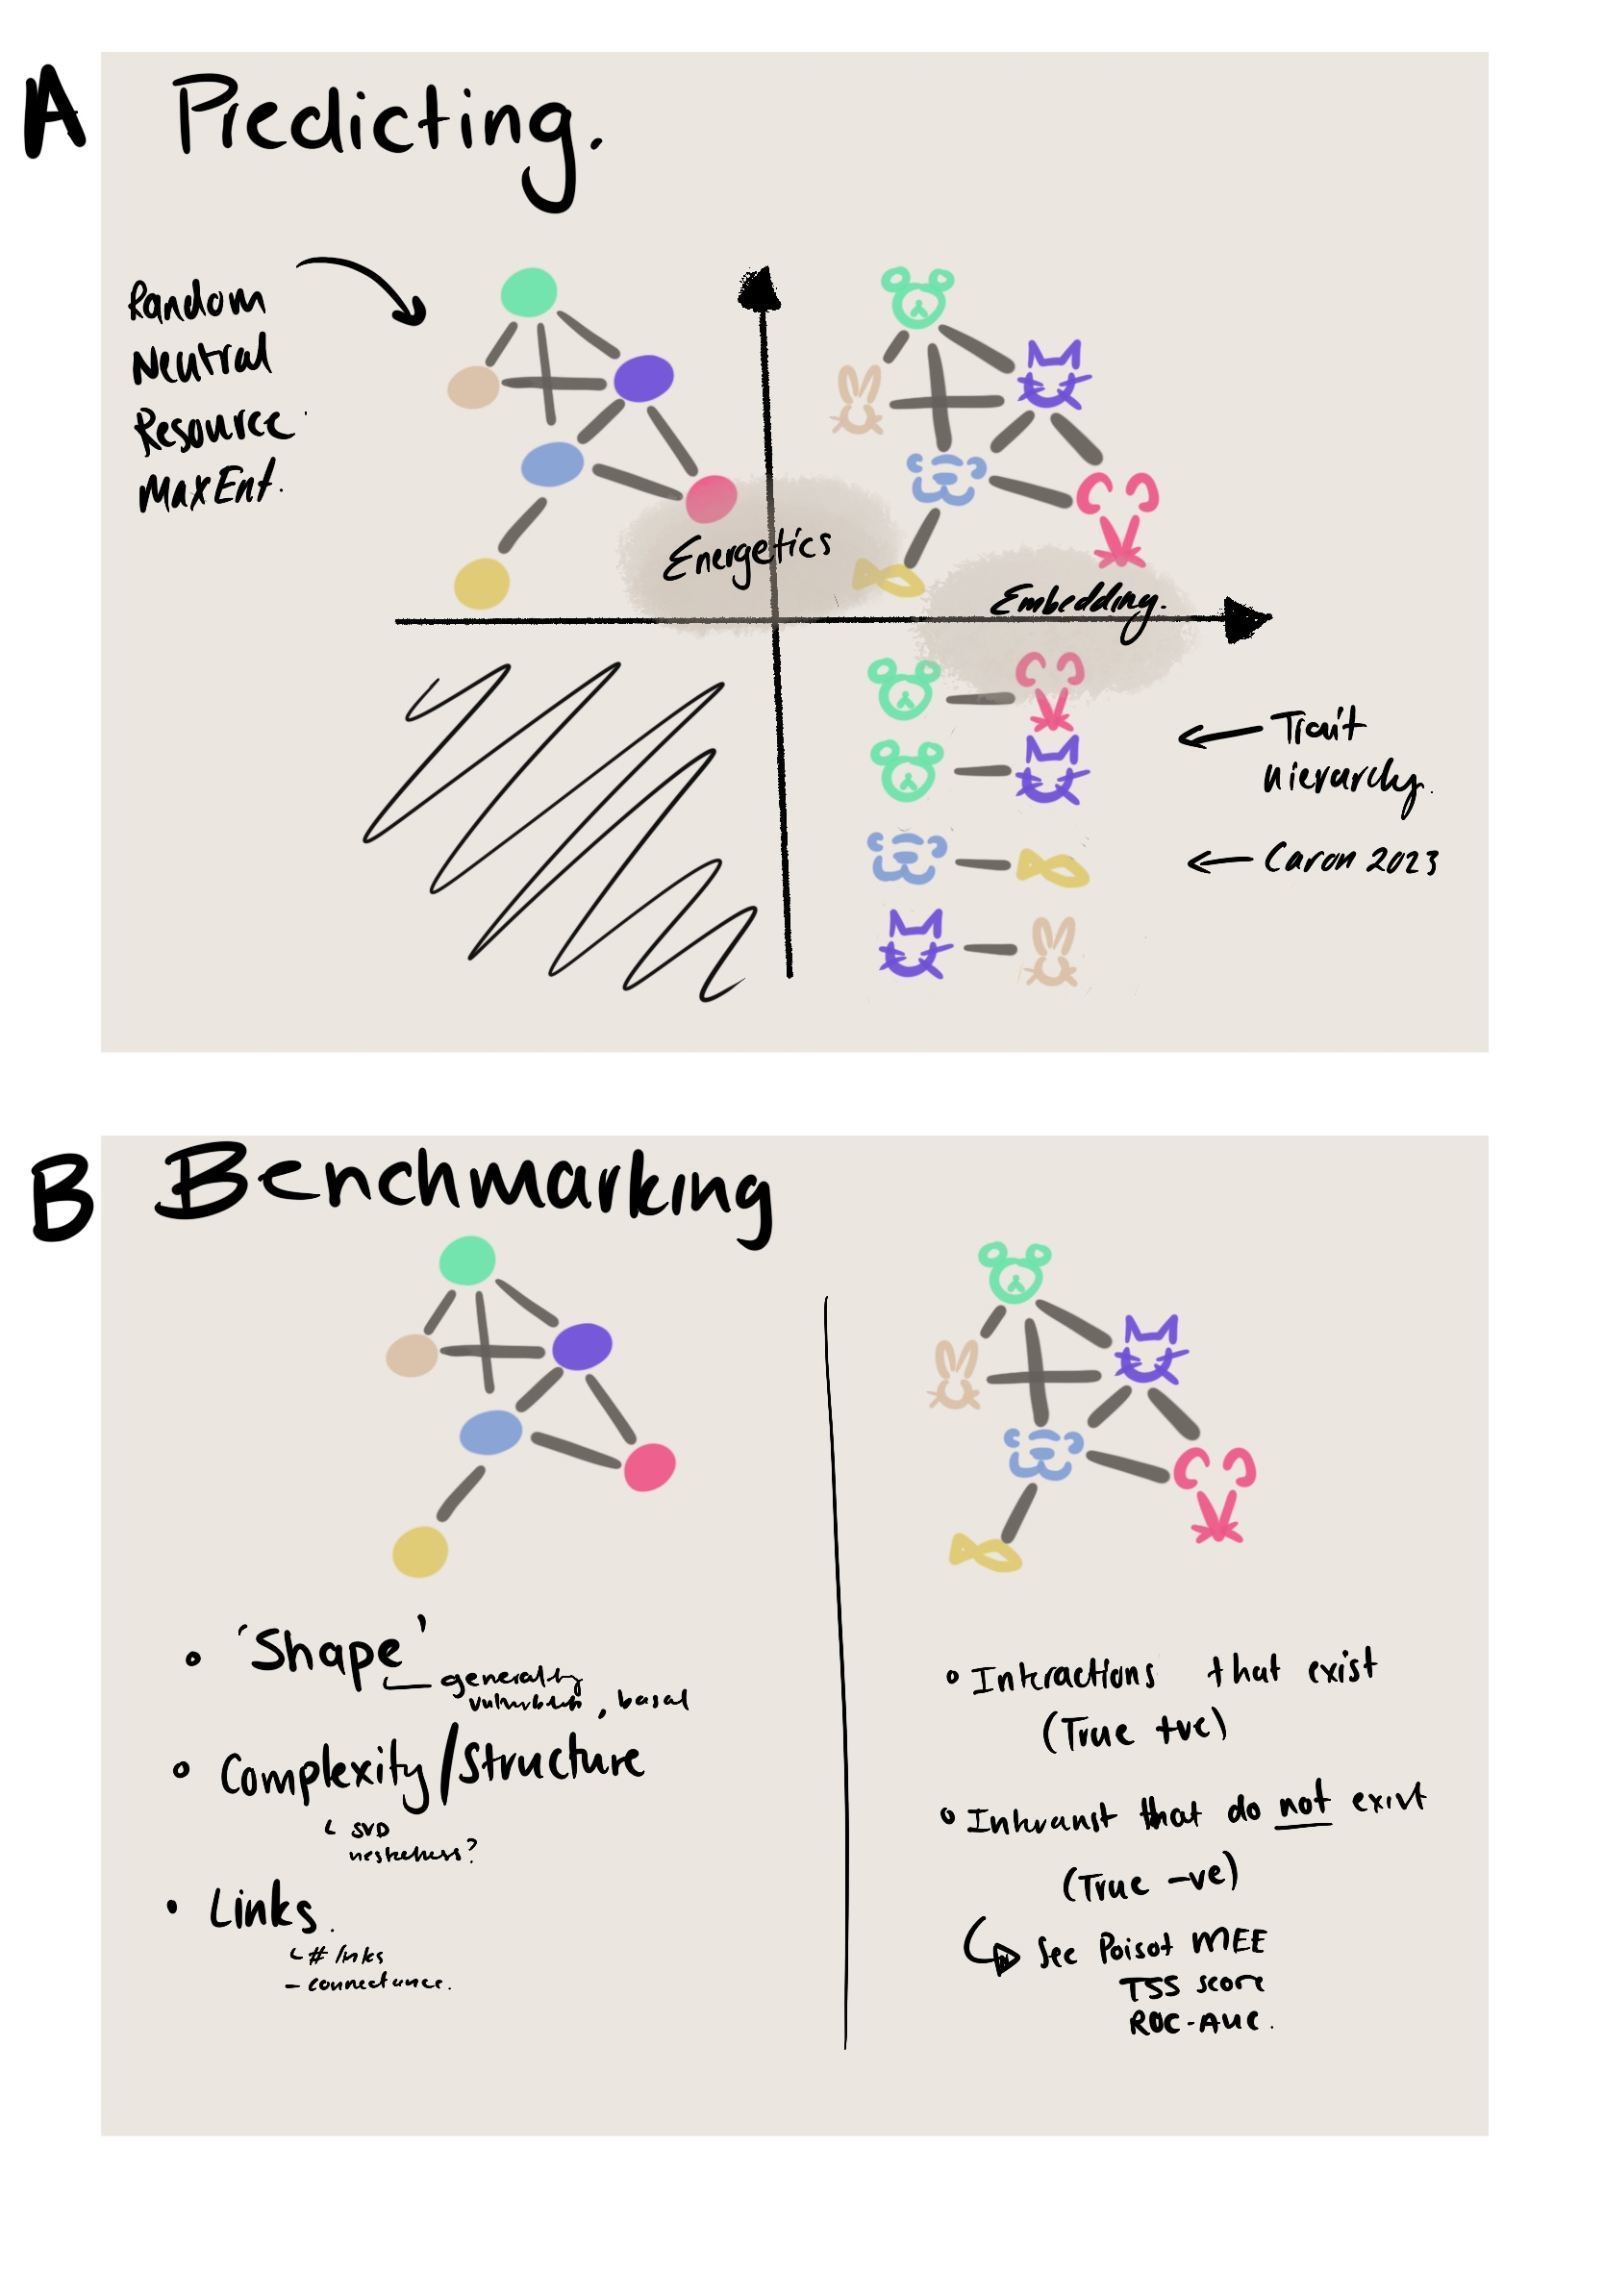
\includegraphics{images/concept.jpeg}

}

\caption{\label{fig-concept}Conceptual figure of the `network
prediction'. Panel A shows where the model families fall in the the
context of being models that predict networks or models that predict
interactions space. Panel B serves to highlight the characteristics one
might like to `test'/benchmark for a model based on it being either a
network or interaction predicting model}

\end{figure}%

\begin{figure}[H]

{\centering 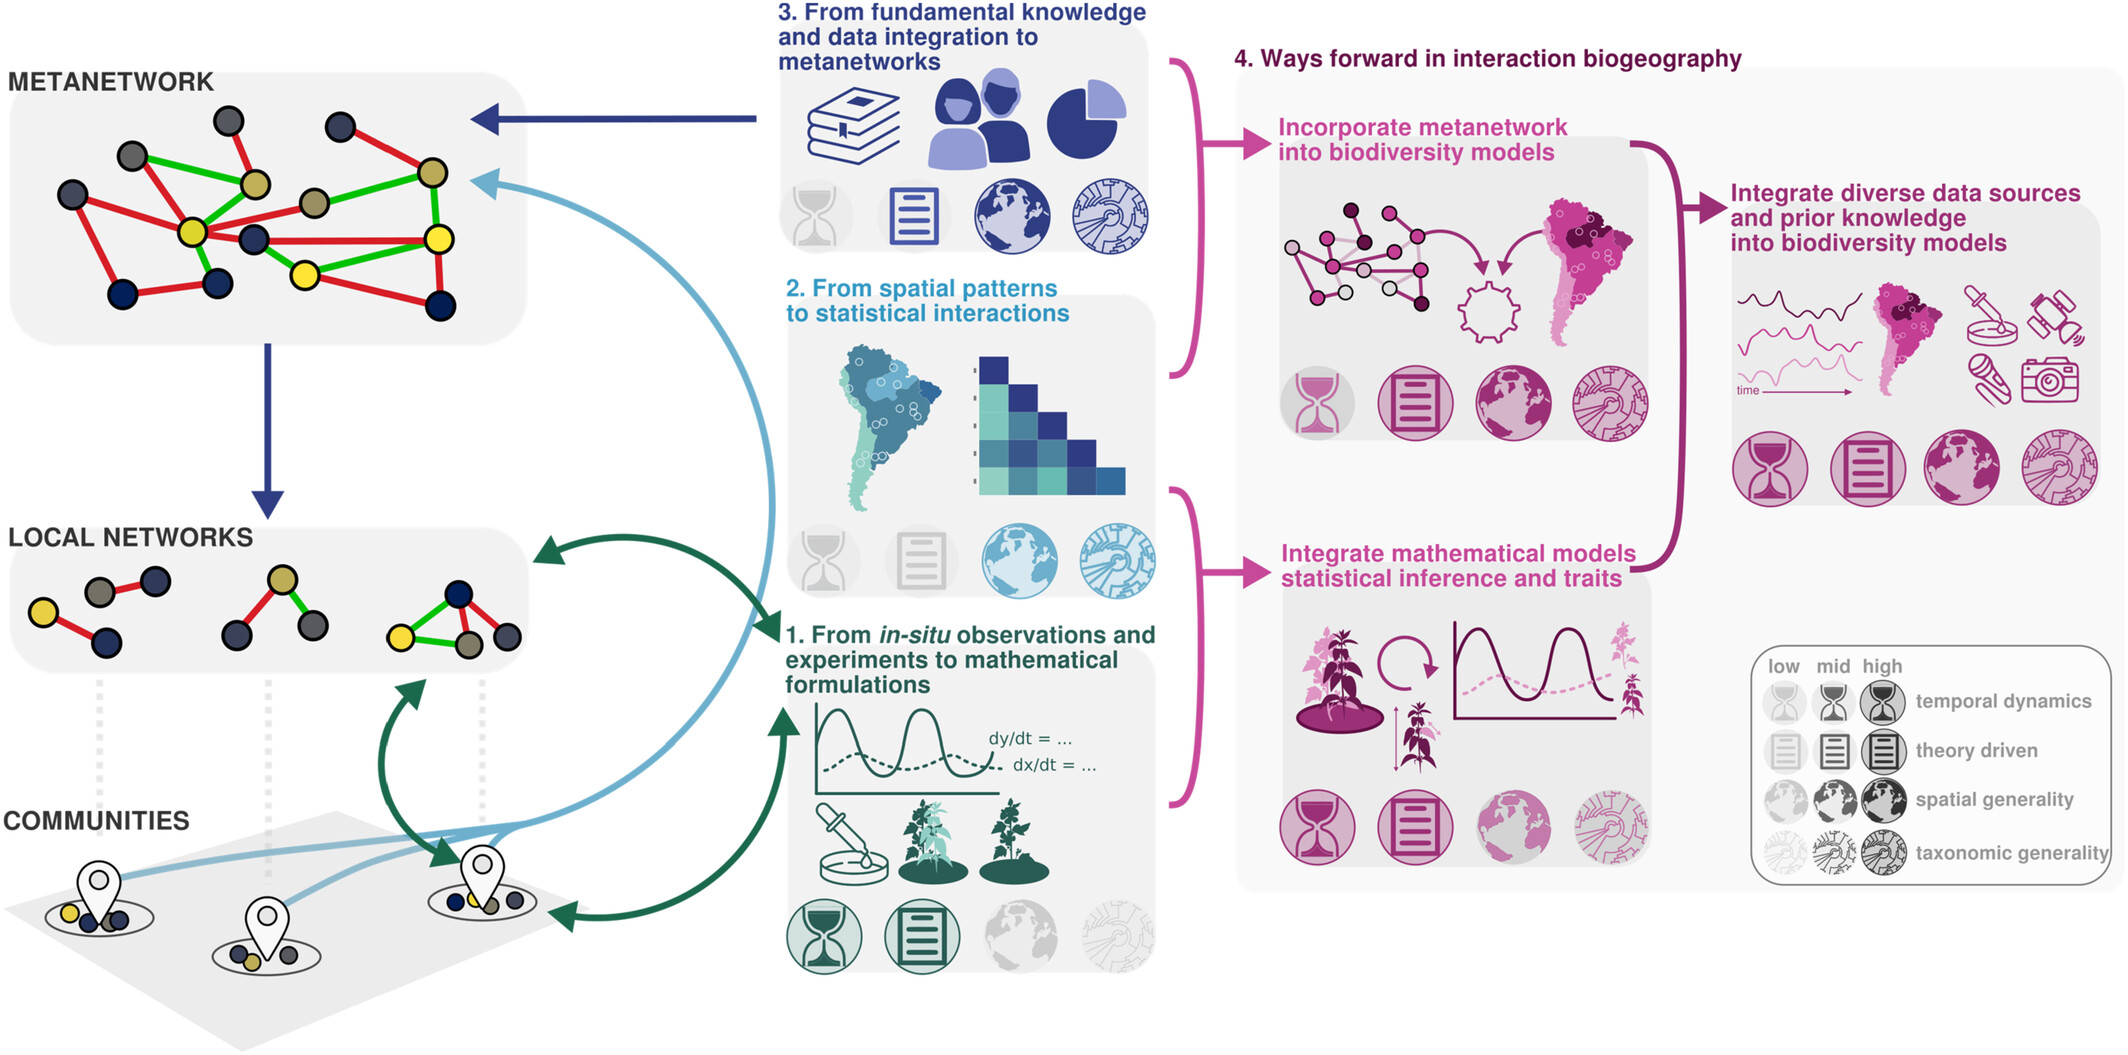
\includegraphics{images/thullier_2023_concept.jpeg}

}

\caption{I like the use of the different source indicator items (not too
dissimilar from Tall Tom's nature paper but also different). This is
from Thuiller et al. (2024)}

\end{figure}%

\textbf{Null models:} The interactions between species occurs regardless
of the identity of the species (\emph{i.e.,} species have no agency) and
links are randomly distributed throughout the network. There is however
the assumption that a network will be constrained by the number of
links. Type I (Fortuna \& Bascompte, 2006), where interactions happen
proportionally to connectance and Type II (Bascompte et al., 2003),
where interactions happen proportionally to the joint degree of the two
species involved. These two models are equivalent to the Erdos-Renyi and
Configuration models (Newman, 2010) respectively (check that though).

\textbf{Neutral models:} Based on the theory that interactions occur as
the result of the abundance of species (\emph{i.e.,} the species still
has no agency but its abundance does?). See Pomeranz et al. (2019)

\textbf{Resource models:} Based on the idea that networks follow a
trophic hierarchy and that species interactions can be determined using
a single dimension {[}the ``niche axis''; Allesina et al. (2008){]}.
Essentially these models can be viewed as being based on the idea of
resource partitioning (niches) along a one-dimensional resource and that
the number of links scale with species richness (linear link scaling).
That is, there is some sort of hierarchical feeding based on how a
`resource' is partitioned. Broadly this family consists of three core
models; the cascade model (Joel E. Cohen et al., 1990), which rests on
the idea that species feed on one another in a hierarchical manner; the
niche model (Williams \& Martinez, 2000), broadly all species are
randomly assigned a `feeding niche' and all species that fall in this
niche can be consumed by that species; and the nested hierarchy model
(Cattin et al., 2004), which adds some component of phylogenetic
clustering/signal\ldots{} so not a single dimension? \textbf{TODO}.
Williams \& Martinez (2008) provides a broader overview of some of the
variations in these models as well as comparison between them regarding
their ability to retrieve elements of networks structure (see also
Allesina et al. (2008)).

\textbf{Generative models:} (this is maybe a bit of a bold term to use).
MaxEnt (Banville et al., 2023), (maybe) stochastic block (Xie et al.,
2017).

\textbf{Feeding models:} Broadly this family of models is rooted in
feeding theory and allocates the links between species based on
energetics, which predicts the diet of a consumer based on energy
intake. This means that the model is focused on predicting not only the
number of links in a network but also the arrangement of these links
based on the diet breadth of a species. The diet breadth model
(Beckerman et al., 2006) as well as its allometrically scaled cousin the
allometric diet breadth model (ADBM) (Petchey et al., 2008) determine
links between species based on the energetic content, handling time, and
density of species. See also DeAngelis et al. (1975)

\begin{quote}
Gravel et al. (2013) also poses an interesting cross-over between the
adbm and niche model.
\end{quote}

\textbf{Binary classifiers:} The task of predicting if an interaction
will occur between a species pair is treated as a statistical binary
classification task, where the task is to correlate `real world'
interaction data with a suitable ecological proxy for which data is more
widely available (\emph{e.g.,} traits). Model families often used
include generalised linear models (\emph{e.g.,} Caron et al., 2022),
random forest (\emph{e.g.,} Llewelyn et al., 2023), trait-based k-NN
(\emph{e.g.,} Desjardins-Proulx et al., 2017), and Bayesian models
(Cirtwill et al., 2019; \emph{e.g.,} Eklöf et al., 2013). See Pichler et
al. (2020) for a more detailed overview on the performance of machine
learning and statistical approaches for inferring trait-trait
relationships.

\textbf{Graph embedding:} This family of approaches has been extensively
discussed in Strydom et al. (2023) but can be broadly explained as an
approach that estimates latent features from observed networks that can
be used to predict interactions. Strydom et al. (2022) uses a transfer
learning framework (specifically using a random dot product graph for
embedding) based around the idea that interactions are evolutionarily
conserved and that we can use known networks, and phylogenetic
relationships, to predict interactions for a given species pool.
\textbf{TODO} Log-ratio (Rohr et al., 2010)

\textbf{Trait matching:} Interactions are determined by a series of
`feeding rules', whereby the interaction between a species pair will
only occur if all feeding rules are met. These rules are determined on
an \emph{a priori} basis using expert/ecological knowledge to determine
the underlying feeding hierarchy using ecological proxies
(Morales-Castilla et al., 2015). For example the Paleo Foodweb Inference
Model (PFIM, Shaw et al., 2024) uses a series of rules for a set of
trait categories (such as habitat and body size) to determine if an
interaction can occur between a species pair. What sets this family of
models apart from \textbf{expert knowledge} ones is that there is a
formalisation of the feeding rules and thus there is some ability to
transfer these rules to different communities.

\textbf{Expert knowledge:} Not so much about empirical observations but
more the value of `local' knowledge and having specific individuals
sitting around a table and assigning a value of how confident they are
that a specific species pair are likely to interact (\emph{e.g.,}
Jennifer A. Dunne et al., 2008), this has the added advantage that
interactions can be scored in a more categorical as opposed to binary
fashion, \emph{e.g.,} Maiorano et al. (2020) score interactions as
either obligate (typical food resources) or occasional (opportunistic
feeding) interactions. I feel like its worth also mentioning downfalls
\emph{a la} Brimacombe et al. (2023)\ldots{}

\textbf{Data scavenging:} There are also a lot of published
\emph{interaction} data that are publicly available \emph{e.g.,} the
Global Biotic Interactions (GloBI) database (Poelen et al., 2014) and
these can also be used to construct an interaction network by mining
these sources to look for interactions for specific species pairs. This
is done by matching species pairs against those within a dataset of
trophic interactions to determine if an interaction is present or absent
between the two species (\emph{e.g.,} the WebBuilder tool developed by
Gray et al., 2015). It is important to note that this methodology is
only going to be able to infer observations that have been recorded in
the field, and given the relative scarcity {[}\emph{I say Poisot et al.
(2021) but that's more an overview of complete networks but one can also
get pairwise interactions from these types of data so I feel like its
okay?}{]} and localised sampling of these types of datasets it is very
likely that there will be many false negatives (missing pairwise
interactions) using this approach.

\textbf{Co-occurrence:} Trying to infer interactions from the
co-occurrence patterns of species pairs within the community
\emph{e.g.,} the geographical lasso (Ohlmann et al., 2018). This (for
me) seems fundamentally flawed and Blanchet et al. (2020) seems to agree
with me at least a little bit.

\section{Model benchmarking}\label{model-benchmarking}

\begin{itemize}
\item
  `Testing' the performance of a model is going to depend on some of the
  core limitations of the model itself thus it makes sense to think of
  two sets benchmarking rules for network and interaction prediction
  models respectively (see Figure~\ref{fig-concept} panel B).
\item
  When it comes to network models we are concerned with the
  `preservation' of structure and distribution of links across the
  network. For interaction models we want to ensure that we are able to
  retrieve interactions that really exist but also those that cannot
  exist (\emph{sensu} forbidden links Jordano (2016b))
\end{itemize}

\begin{quote}
``As long as these predictions are not perfect, some interactions will
be predicted at the `wrong' position in the network; these measures
cannot describe the structural effect of these mistakes. On the other
hand, measures of network structure can have the same value with
interactions that fall at drastically different positions; this is in
part because a lot of these measures covary with connectance, and in
part because as long as these values are not 0 or their respective
maximum, there is a large number of network configurations that can have
the same value.'' - Poisot (2023)
\end{quote}

\subsection{Benchmarking network
models}\label{benchmarking-network-models}

\begin{itemize}
\item
  Maybe look at some of the historic papers that compare some of the
  `resource models'
\item
  See also Allesina et al. (2008) and the likelihood function that they
  use for model selection
\item
  Look at Vermaat et al. (2009)
\end{itemize}

\begin{quote}
``Possibly, the most striking caveat of the use of summary statistics is
that it cannot tell us whether or not a model is able to fully replicate
empirical networks.'' - Allesina et al. (2008)
\end{quote}

\subsection{Benchmarking interaction
models}\label{benchmarking-interaction-models}

\begin{itemize}
\item
  Main concern with predicting interactions is that we want to test the
  `quality' of the links we are predicting (both true positives and true
  negatives), but the inherit sparsity (meaning high class imbalance)
  means that we also need to look at the balance of these predictions.
\item
  ``Both precision and recall may be useful in cases where there is
  imbalanced data. However, it may be valuable to prioritize one over
  the other in cases where the outcome of a false positive or false
  negative is costly.''
\item
  Caveat regarding the use of real world interaction data both for
  training and validating predictions? \emph{e.g.,} Poisot, Ouellet, et
  al.~et al 2021 and Catchen et al 2023
\item
  See Poisot (2023)

  \begin{itemize}
  \item
    skill (ability to make the right prediction; evaluate whether low
    prevalence can lull us into a false sense of predictive accuracy)
  \item
    bias (trends towards systematically over-predicting one class)
  \item
    class imbalance (the relative number of cases representing
    interactions)
  \end{itemize}
\item
  ``These results suggest that learning from a dataset with very low
  connectance can be a different task than for more connected networks:
  it becomes increasingly important to capture the mechanisms that make
  an interaction exist, and therefore having a slightly more biased
  training dataset might be beneficial. As connectance increases, the
  need for biased training sets is less prominent, as learning the rules
  for which interactions do not exist starts gaining importance''
\item
  Maybe also looking at how well a model can recover `missing links'
  \emph{i.e.,} false negatives \emph{sensu} what we did in Strydom et
  al. (2022)
\item
  Need to discuss the key differences and implications between
  predicting a metaweb (\emph{sensu} Jennifer A. Dunne (2006)) and a
  network realisation. Maybe also Poisot et al. (2015) that discuss how
  the local factors are going to play a role.
\end{itemize}

\section{Data \& Methods}\label{sec-data-methods}

\subsection{Selecting models}\label{selecting-models}

This section depends on if we go the family route and where we introduce
them. But a more extended description of each model can be found in the
\texttt{Extended\ Model\ Description} notebook (I'm trying to work out
how to embed this\ldots)

I know tables are awful but in this case they may make more sense. Also
I don't think I'm at the point where I can say that the table is
complete/comprehensive but it getting there Not sure about putting in
some papers that have used the model - totes happy to drop those I
think\ldots{}

\begin{longtable}[]{@{}
  >{\raggedright\arraybackslash}p{(\columnwidth - 16\tabcolsep) * \real{0.1111}}
  >{\raggedright\arraybackslash}p{(\columnwidth - 16\tabcolsep) * \real{0.1111}}
  >{\raggedright\arraybackslash}p{(\columnwidth - 16\tabcolsep) * \real{0.1111}}
  >{\raggedright\arraybackslash}p{(\columnwidth - 16\tabcolsep) * \real{0.1111}}
  >{\raggedright\arraybackslash}p{(\columnwidth - 16\tabcolsep) * \real{0.1111}}
  >{\raggedright\arraybackslash}p{(\columnwidth - 16\tabcolsep) * \real{0.1111}}
  >{\raggedright\arraybackslash}p{(\columnwidth - 16\tabcolsep) * \real{0.1111}}
  >{\raggedright\arraybackslash}p{(\columnwidth - 16\tabcolsep) * \real{0.1111}}
  >{\raggedright\arraybackslash}p{(\columnwidth - 16\tabcolsep) * \real{0.1111}}@{}}
\caption{Lets make a table that gives an overview of the different model
families and some of their features. \emph{A column that captures naïve
vs a priori knowledge of interactions/structure i.e., a `parameter' of
sorts?}}\label{tbl-history}\tabularnewline
\toprule\noalign{}
\begin{minipage}[b]{\linewidth}\raggedright
Model family
\end{minipage} & \begin{minipage}[b]{\linewidth}\raggedright
Theory
\end{minipage} & \begin{minipage}[b]{\linewidth}\raggedright
Network predicted
\end{minipage} & \begin{minipage}[b]{\linewidth}\raggedright
Links predict
\end{minipage} & \begin{minipage}[b]{\linewidth}\raggedright
Make `\emph{de novo}' predictions (node/species identity)
\end{minipage} & \begin{minipage}[b]{\linewidth}\raggedright
Needs (minimum)
\end{minipage} & \begin{minipage}[b]{\linewidth}\raggedright
Assembly mechanism
\end{minipage} & \begin{minipage}[b]{\linewidth}\raggedright
Constraints
\end{minipage} & \begin{minipage}[b]{\linewidth}\raggedright
Interaction
\end{minipage} \\
\midrule\noalign{}
\endfirsthead
\toprule\noalign{}
\begin{minipage}[b]{\linewidth}\raggedright
Model family
\end{minipage} & \begin{minipage}[b]{\linewidth}\raggedright
Theory
\end{minipage} & \begin{minipage}[b]{\linewidth}\raggedright
Network predicted
\end{minipage} & \begin{minipage}[b]{\linewidth}\raggedright
Links predict
\end{minipage} & \begin{minipage}[b]{\linewidth}\raggedright
Make `\emph{de novo}' predictions (node/species identity)
\end{minipage} & \begin{minipage}[b]{\linewidth}\raggedright
Needs (minimum)
\end{minipage} & \begin{minipage}[b]{\linewidth}\raggedright
Assembly mechanism
\end{minipage} & \begin{minipage}[b]{\linewidth}\raggedright
Constraints
\end{minipage} & \begin{minipage}[b]{\linewidth}\raggedright
Interaction
\end{minipage} \\
\midrule\noalign{}
\endhead
\bottomrule\noalign{}
\endlastfoot
null & Network structure is random & structure & & no & network (species
agnostic) & random & link & binary \\
neutral & Network structure is random, but species abundance plays a
role & structure & & yes & abundance, number of links & mass effect &
link & binary \\
resource & Networks are interval, species can be ordered on a `niche
axis' & structure & flow of biomass (resource?) & no & richness,
connectance & `random' & link & binary \\
generative & Networks are determined by their structural features &
structure & & no & network (species agnostic) & `random' & & binary \\
energetic & Interactions are determined by foraging theory (feeding
links) & interactions & flow of energy & yes & body size & deterministic
& energy & \\
graph embedding & Interactions can be predicted from the latent traits
of networks & interactions & potential feeding links & yes &
interactions, phylogenetic tree, list of target species (species pool) &
& & probabilistic \\
trait matching & Interactions can be inferred by a mechanistic
framework/relationships & interactions & potential feeding links & yes &
prior (expert) knowledge of trait hierarchy/relationships, traits, list
of target species (species pool) & mechanistic & trait matching
(\emph{sensu} forbidden links in a way) & \\
binary classifiers & Interactions can be predicted by learning the
relationship between interactions and ecologically relevant predictors &
interactions & potential feeding links & yes & interactions, traits,
list of target species (species pool) & statistical & & \\
expert knowledge & `Boots on the ground' ecological knowledge and
observations & interactions & potential feeding links & yes & list of
target species (species pool) & mechanistic & forbidden links & \\
data scavenging & Webscraping to create networks from online databases &
interactions & potential feeding links & no & list of target species
(species pool) & & & binary \\
co-occurrence & co-occurrence patterns arise from interactions so we can
use these patterns to reverse engineer the interactions & co-occurrence
links? (or am I being a bit too mean here) & association links & &
co-occurrence (so a species list?) & & & \\
\end{longtable}

\subsection{Datasets used}\label{datasets-used}

\subsubsection{Mangal networks}\label{mangal-networks}

We queried the Mangal (Poisot, Baiser, et al., 2016) database and
extracted a total of \textbf{TODO} networks. {[}\emph{Some sort of
summary as to the geographic/taxonomic range??{]}} Although these
networks represent a high volume of interaction data they do not have
accompanying `metadata' that we would need for some of the more
data-hungry model families (\emph{e.g.,} local abundance), the Mangal
networks were used to provide the `starting values' for the random,
resource, and generative families. This allows us to generate a large
number of different networks that we can use to compare and contrast the
performance of the various model families (see
Section~\ref{sec-model-benchmarking} for a more detailed breakdown). For
each network from Mangal we generated \textbf{TODO} versions of that
network using each model family.

\begin{quote}
``These complex food webs differ in their level of resolution and
sampling effort, which may introduce noise in the estimation of their
properties, especially given their large number of interacting elements.
However, because our MaxEnt models are applied on imperfect data, they
aim at reproducing the sampled structure of food webs, not their actual
structure.'' - Banville et al. (2023) (something to think about\ldots)
\end{quote}

\subsubsection{Empirical networks}\label{empirical-networks}

`Elite' number of datasets for interaction models

Although the availability of empirical interaction data is growing as
techniques begin to improve and grow (Pringle \& Hutchinson, 2020), we
still lack a way to define what is the `ideal' interaction dataset.

New Zealand dataset(s): Pomeranz et al. (2019)

\begin{quote}
Here I think we need to span a variety of domains, at minimum aquatic
and terrestrial but maybe there should be a `scale' element as well
\emph{i.e.,} a regional and local network. I think there is going to be
a `turning point' where structural will take over from mechanistic in
terms of performance. More specifically at local scales bioenergetic
constraints (and co-occurrence) may play a bigger role in structuring a
network whereas at the metaweb level then mechanistic may make more
(since by default its about who can potentially interact and obviously
not constrained by real-world scenarios) \emph{sensu} Caron et al.
(2024). Although having said that I feel that contradicts the idea of
backbones (\emph{sensu} Bramon Mora (sp?) et al \& Stouffer et al) But
that might be where we get the idea of core \emph{structure} vs
something like linkage density. So core things like trophic level/chain
length will be conserved but connectance might not (I think I understand
what I'm trying to say here)
\end{quote}

I think we should also use the Jennifer A. Dunne et al. (2008) work.
Because 1) it gives the paleo-centric methods their moment in the sun
and 2) I think it also brings up the interesting question of can we use
modern structure to predict past ones?

\subsection{Model benchmarking}\label{sec-model-benchmarking}

For now the (still essentially pending) workflow/associated code can be
found at the following repository
\href{https://github.com/BecksLab/topology_generators}{BecksLab/topology\_generators}.
This will reflect that which is shown in panel \emph{B} of
Figure~\ref{fig-concept}.

\begin{itemize}
\tightlist
\item
  Data `cost' (some methods might need a lot lot of supporting data vs
  something very light weight)
\item
  I think it would be remiss to not also take into consideration
  computational cost
\item
  Something about the network output - I'm acknowledging my biases and
  saying that probabilistic (or \emph{maybe} weighted) links are the way
\end{itemize}

\subsubsection{Network models}\label{network-models}

Want to compare real vs predicted and then get something that looks like
Figure~\ref{fig-topology}

\begin{itemize}
\item
  connectance, nestedness (Bastolla et al., 2009), modularity (Barber,
  2007), asymmetry (Delmas et al., 2018), and Jaccard network
  dissimilarity (Canard et al., 2014)
\item
  \emph{Shape:} do the models construct tall `pencil' vs flat `pancake'
  networks (Beckerman 2024, pers comms), generality/vulnerability, chain
  length (?)
\item
  \emph{Structure:} Predicting `structure' - SVD (Strydom, Dalla Riva,
  et al., 2021) but maybe something like nestedness as well (?)
\item
  \emph{Links:} are the number of links preserved (most network
  predicting models are to some extend link constrained but useful to
  see)
\item
  \emph{Motifs:} Staniczenko et al. (2010) uses S1, S2, S4, S5 from
  Stouffer et al. (2007)

  \begin{itemize}
  \item
    S1: Number of linear chains
  \item
    S2: Number of omnivory motifs
  \item
    S4: Number of apparent competition motifs
  \item
    S5: Number of direct competition motifs
  \end{itemize}
\end{itemize}

\subsubsection{Interaction models}\label{interaction-models}

\begin{itemize}
\tightlist
\item
  Based on Poisot (2023):

  \begin{itemize}
  \tightlist
  \item
    Precision-Recall (PR-AUC) - performance
  \item
    Matthews correlation coefficient (MCC) - accuracy
  \end{itemize}
\item
  Maybe same measures we use for the network models
\end{itemize}

\subsubsection{Action plan}\label{action-plan}

\begin{enumerate}
\def\labelenumi{\arabic{enumi}.}
\tightlist
\item
  Shortlist/finalise the different topo generators
\item
  collate/translate into \texttt{Julia}

  \begin{itemize}
  \tightlist
  \item
    \emph{e.g.,} some models wil be in SpeciesInteractionNetworks.jl
    (new EcoNet); I know (parts of) the transfer learning stuff is and
    the niche model
  \item
    others will need to be coded out (the more simpler models should be
    easier)
  \end{itemize}
\item
  Curate networks for the different datasets/scenarios we select - I
  feel like there might be some scenarios that we can't do all models
  for all datasets but maybe I'm being a pessimist.

  \begin{itemize}
  \tightlist
  \item
    Need to also think about where one might find the additional data
    for some of the models\ldots{}

    \begin{itemize}
    \tightlist
    \item
      Body size: Herberstein et al. (2022) - Although maybe Andrew has
      strong thotsTM RE the one true body size database to rule them
      all\ldots{}
    \item
      Other trait sources: Wilman et al. (2014) and Jones et al. (2009)
    \item
      This is where we'll get the paleo traits from if I'm correct
      Bambach et al. (2007)
    \item
      Phylogeny stuff: Upham et al. (2019) (what we used for TL but its
      only mammals\ldots) but I'm sure there will be others
    \end{itemize}
  \item
    Also limitation of scope\ldots{} \emph{e.g.,} do we even dare to
    think about including plants/basal producers (see \emph{e.g.,}
    Valdovinos et al. (2023))
  \item
    Taxonomic harmonisation - something to think about and check
  \end{itemize}
\end{enumerate}

\section{Results}\label{results}

Joel E. Cohen et al. (1985) actually tells us that the cascade model
only really works for communities that range from 3-33 species\ldots{}
and Williams \& Martinez (2008) also highlights how structural models
really only work for small communities

\subsection{Qualitative stuff}\label{qualitative-stuff}

Maybe not the best term to use but thinking here about practical
limitations of the different families. This can include thinking about:

\begin{itemize}
\tightlist
\item
  scale limitations (time or space); \emph{e.g.,} a metaweb is going to
  encapsulate but not distinguish between different seasons or locations
\item
  data needed. I think this can be in the form of real world datasets
  (\emph{e.g.,} traits) but also \emph{a priori} knowledge (\emph{e.g.,}
  having to define the constraints of a niche model)
\item
  computational costs
\end{itemize}

\begin{figure}

\centering{

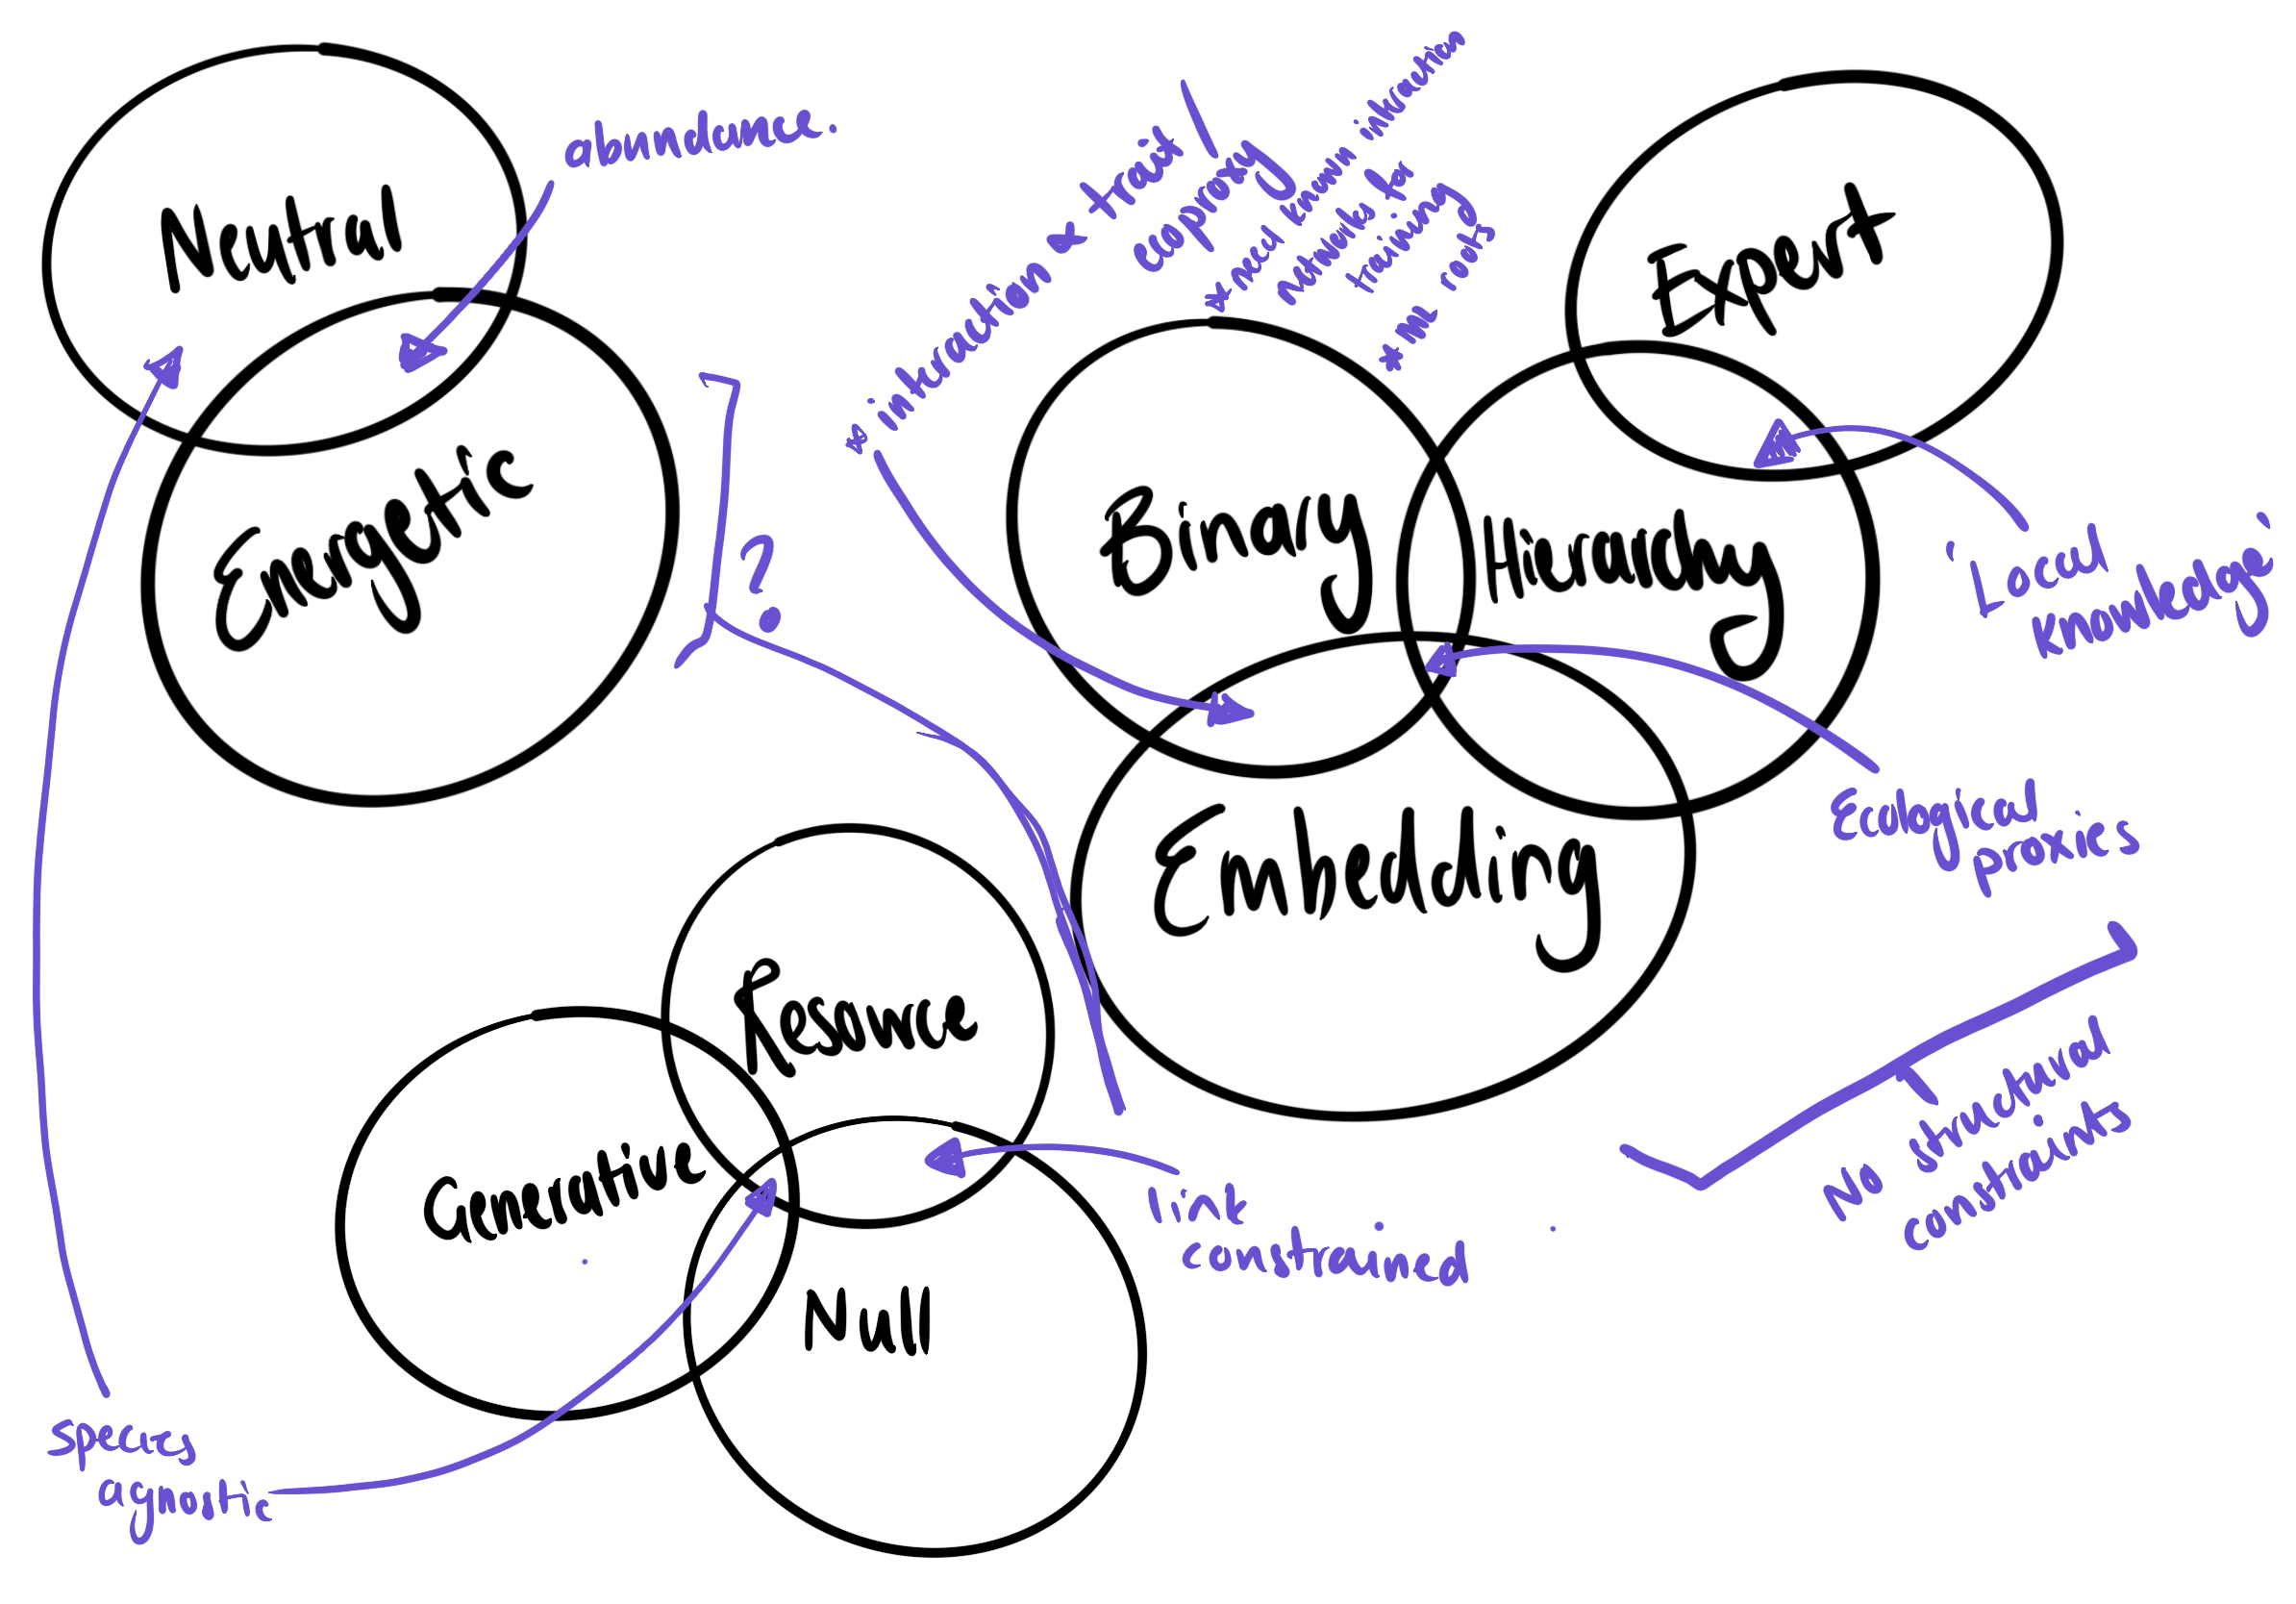
\includegraphics{images/model_venn.png}

}

\caption{\label{fig-venn}I still haven't given up on a sort of venn
diagram idea but maybe it going to be more of a venn-flow chart
hybrid\ldots{}}

\end{figure}%

\begin{figure}

\centering{

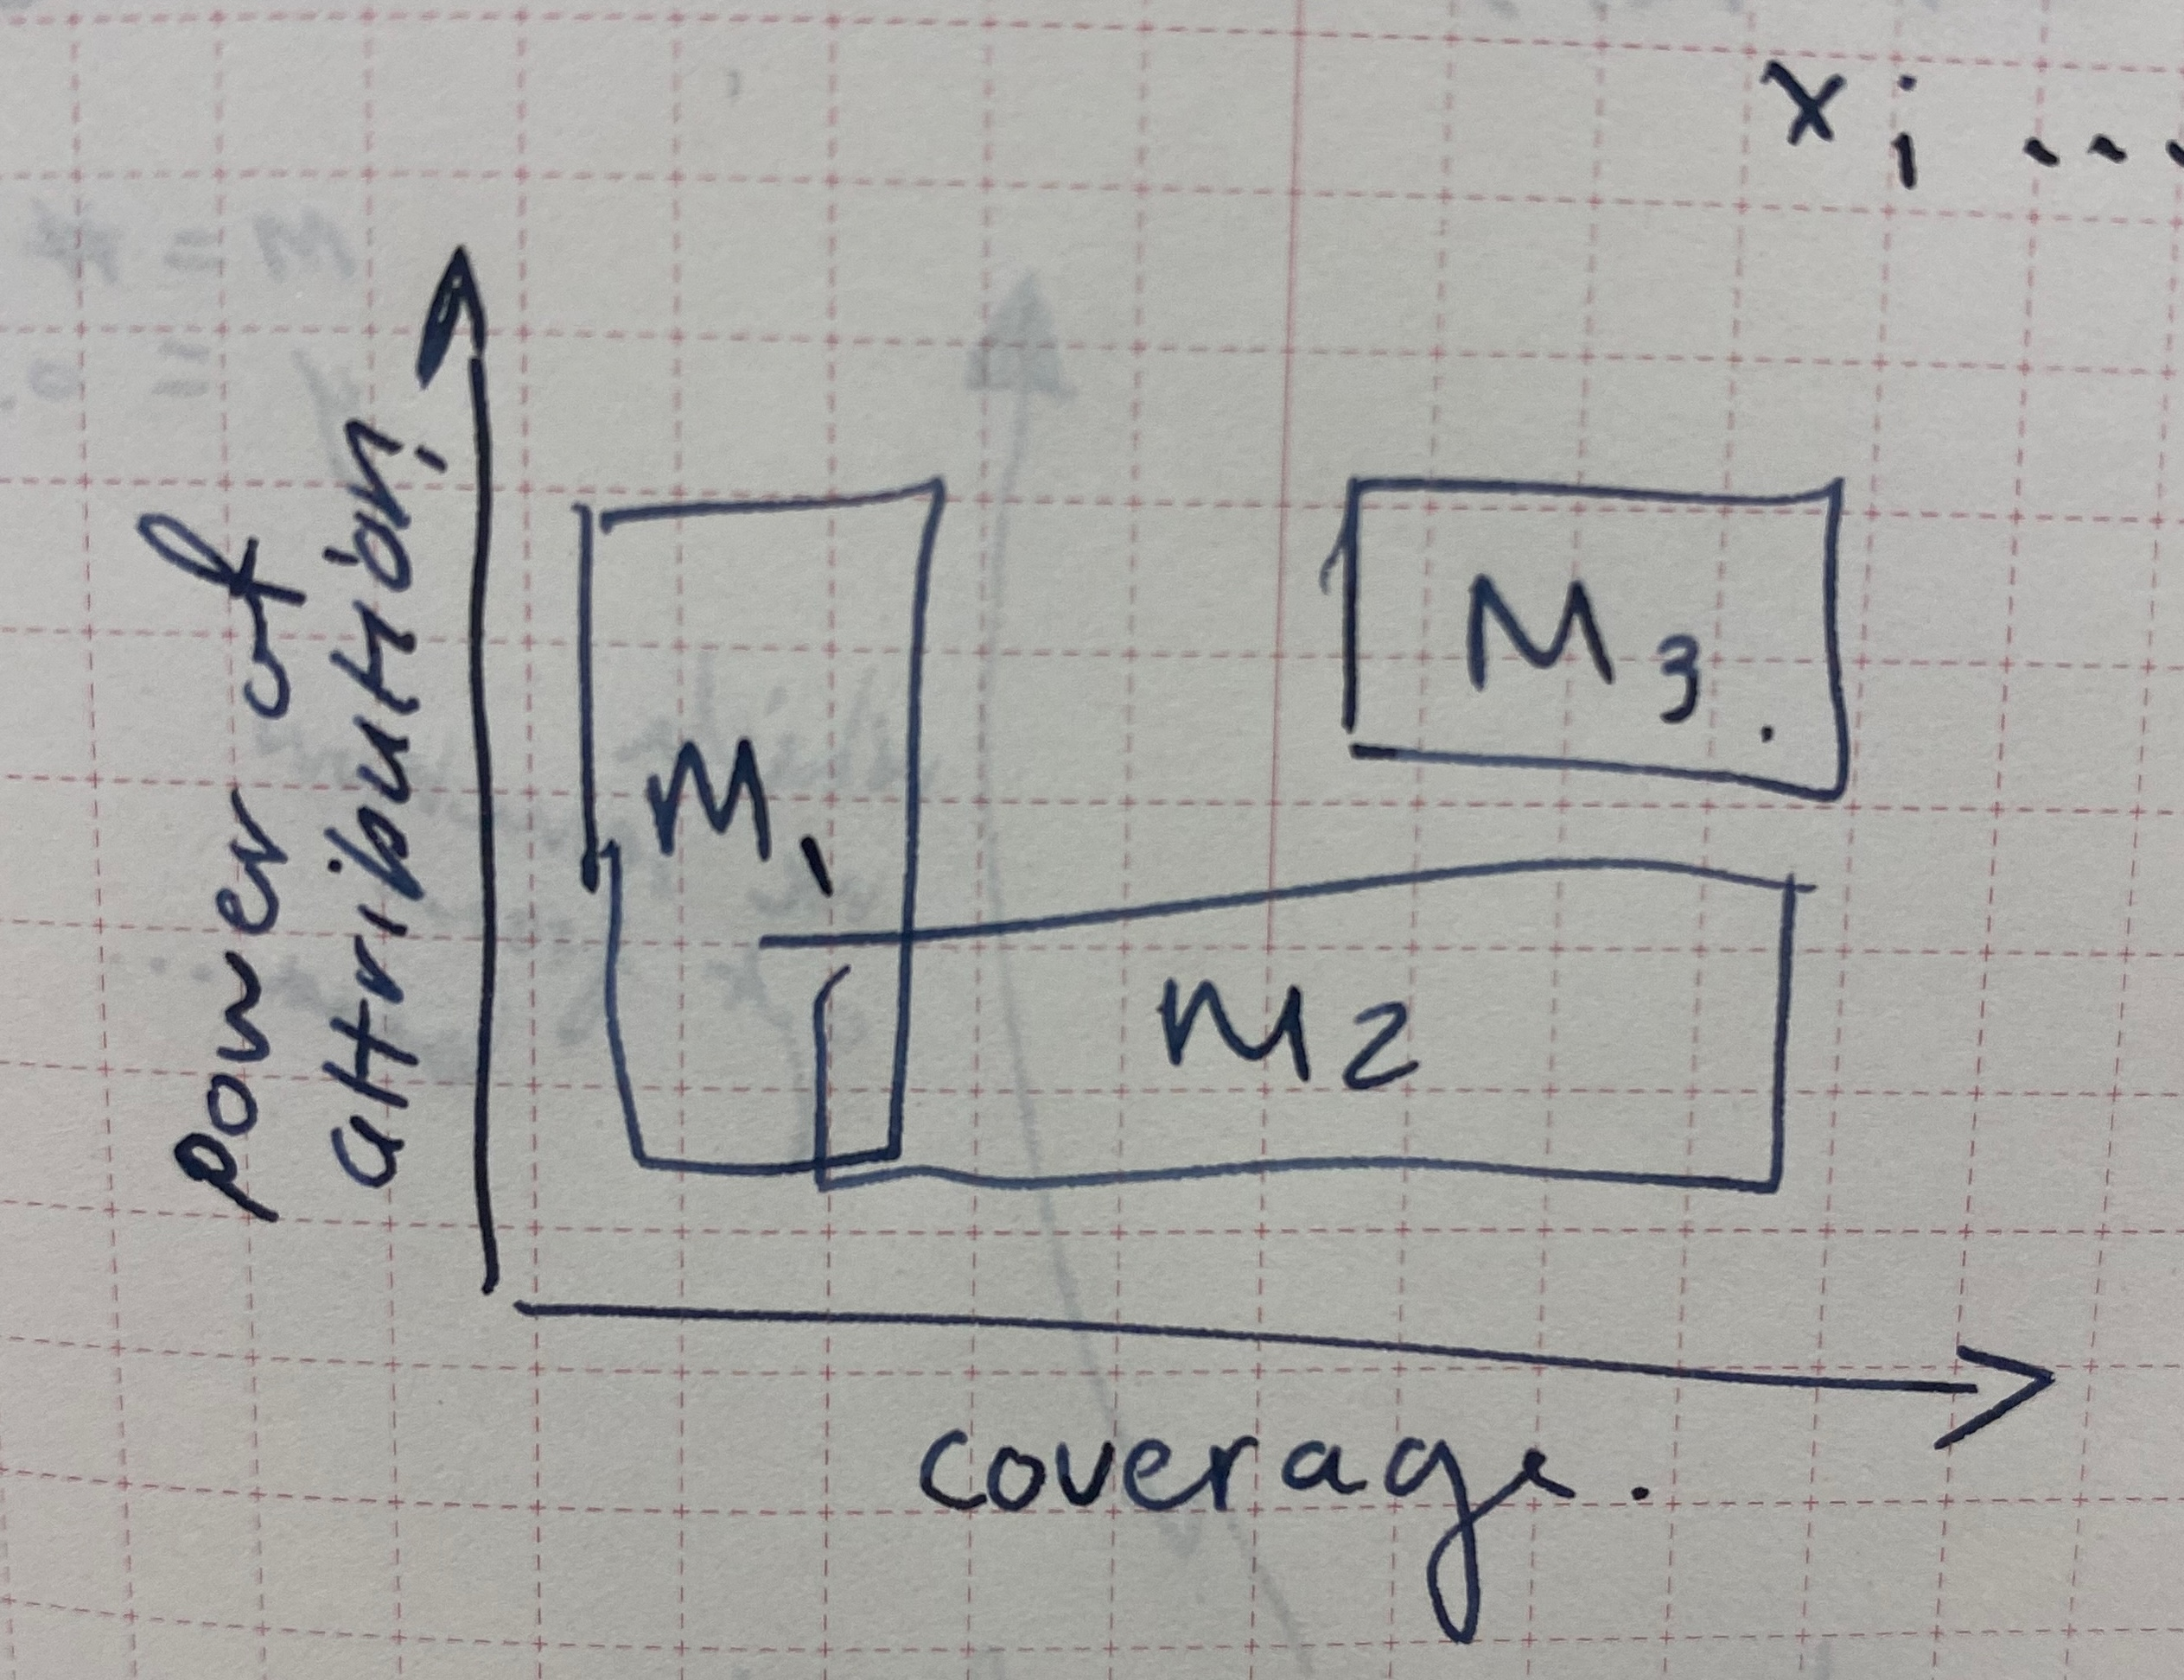
\includegraphics{images/outhwaite_schematic.jpeg}

}

\caption{\label{fig-outhwaite}I like these schematics that Charlie
Outhwaite presented at the EEB seminar (there was a series of them).}

\end{figure}%

\subsection{Quantitative stuff}\label{quantitative-stuff}

\begin{figure}[H]

\centering{

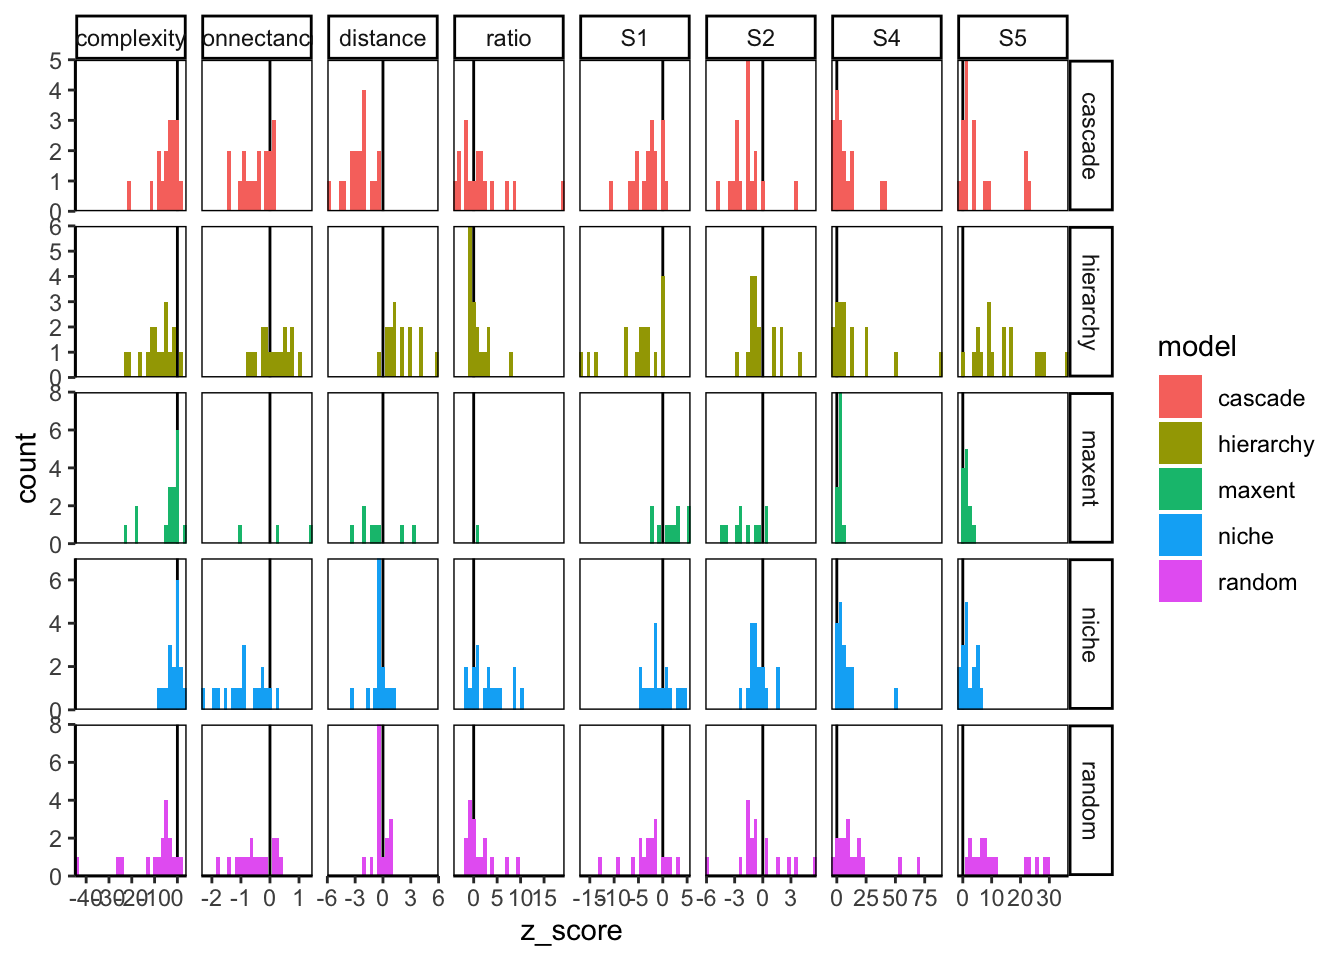
\includegraphics{index_files/figure-latex/notebooks-model_quantitative-fig-topology-output-2.png}

}

\caption{\label{fig-topology}Difference between real and model network
property. S1 - S5 represent the different motif structures identified in
Stouffer et al. (2007).}

\end{figure}%

\textsubscript{Source:
\href{https://BecksLab.github.io/ms_t_is_for_topology/index.qmd.html}{Article
Notebook}}

I really like this way of plotting results from Pichler et al. (2020)

\begin{figure}

\centering{

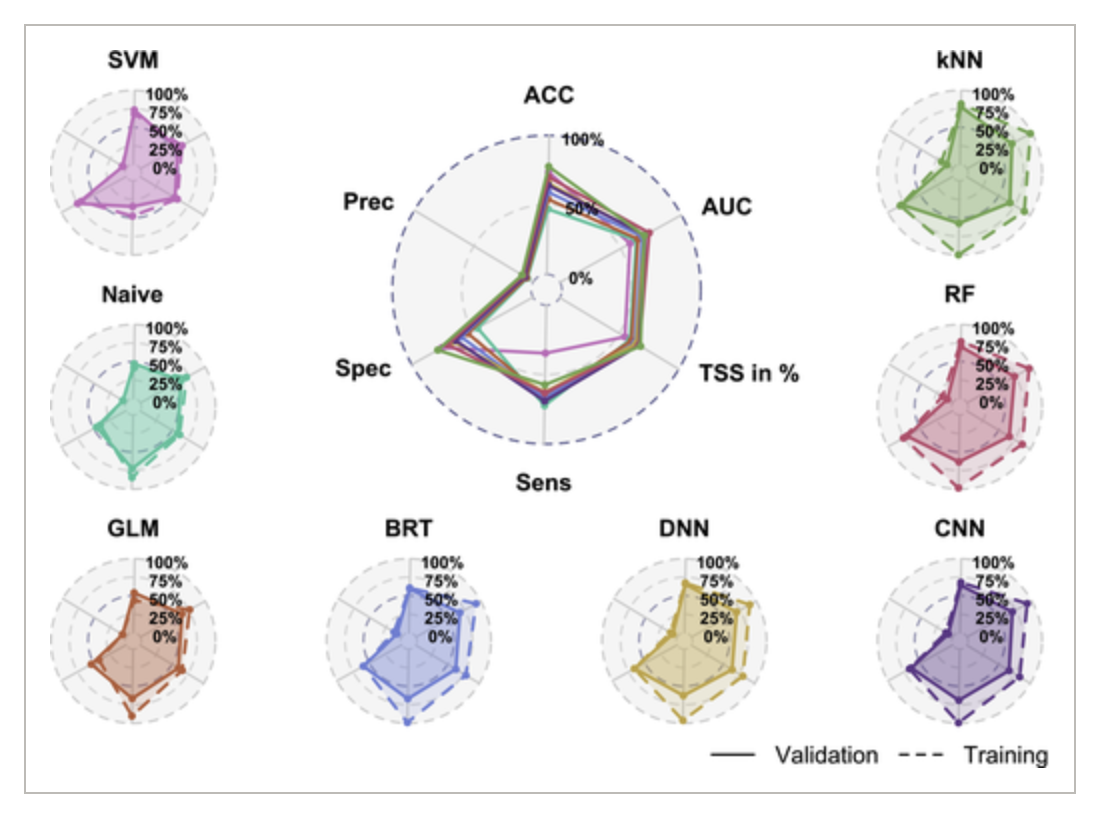
\includegraphics{images/pichler_result.png}

}

\caption{\label{fig-pichler}Cool way to conceptualise results from
Pichler et al. (2020)}

\end{figure}%

\section{Discussion}\label{discussion}

\begin{itemize}
\item
  I think a big take home will (hopefully) be how different approaches
  do better in different situations and so you as an end user need to
  take this into consideration and pick accordingly. I think Petchey et
  al. (2011) might have (and share) some thoughts on this (thanks
  Andrew). I feel like I need to look at Berlow et al. (2008) but maybe
  not exactly in this context but vaguely adjacent.
\item
  An interesting thing to also think about (and arguably it will be
  addressed based on some of the other thoughts and ideas) is data
  dependant and data independent `parametrisation' of the models\ldots{}
\item
  Why do interaction models do so badly at predicting structure? Nuance
  of metaweb vs realisation but also time? At the core of it interaction
  models are trained on existing interaction data; this is data that are
  most likely closer to a metaweb than a local realisation even if they
  are being inventoried at a small scale.

  \begin{itemize}
  \tightlist
  \item
    I think this is sort of the crux of the argument presented in
    Brimacombe et al. (2024)
  \end{itemize}
\end{itemize}

\begin{quote}
\emph{``we highlight an interesting paradox: the models with the best
performance measures are not necessarily the models with the closest
reconstructed network structure.''} - Poisot (2023)
\end{quote}

\begin{itemize}
\item
  \emph{Do we need network models to predict interactions and
  interaction models to predict structure?} (lets not think about that
  too hard or I might just have to sit in silence for a while\ldots)

  \begin{itemize}
  \item
    ``Another argument for the joint prediction of networks and
    interactions is to reduce circularity and biases in the predictions.
    As an example, models like linear filtering generate probabilities
    of non-observed interactions existing, but do so based on measured
    network properties.'' - Strydom, Catchen, et al. (2021)
  \item
    Aligning (dove-tailing) with this the idea of ensemble modelling as
    presented by Becker et al. (2022)
  \end{itemize}
\item
  It will be interesting to bring up the idea that if a model is missing
  a specific pairwise link but doing well at the structural level then
  when does it matter?
\item
  Close out with a call to action that we have models that predict
  networks very well and models that predict interactions very well but
  nothing that is doing well at predicting both - this is where we
  should be focusing our attention when it comes to furthering model
  development. (we need models that will fill the space in the top right
  quadrant of panel A in Figure~\ref{fig-concept})
\end{itemize}

\section*{References}\label{references}
\addcontentsline{toc}{section}{References}

\vspace{1em}

\textsubscript{Source:
\href{https://BecksLab.github.io/ms_t_is_for_topology/index.qmd.html}{Article
Notebook}}

\phantomsection\label{refs}
\begin{CSLReferences}{1}{0}
\bibitem[\citeproctext]{ref-allesinaGeneralModelFood2008}
Allesina, S., Alonso, D., \& Pascual, M. (2008). A {General Model} for
{Food Web Structure}. \emph{Science}, \emph{320}(5876), 658--661.
\url{https://doi.org/10.1126/science.1156269}

\bibitem[\citeproctext]{ref-bambachAutecologyFillingEcospace2007}
Bambach, R. K., Bush, A. M., \& Erwin, D. H. (2007). Autecology and the
{Filling} of {Ecospace}: {Key Metazoan Radiations}.
\emph{Palaeontology}, \emph{50}(1), 1--22.
\url{https://doi.org/10.1111/j.1475-4983.2006.00611.x}

\bibitem[\citeproctext]{ref-banvilleWhatConstrainsFood2023}
Banville, F., Gravel, D., \& Poisot, T. (2023). What constrains food
webs? {A} maximum entropy framework for predicting their structure with
minimal biases. \emph{PLOS Computational Biology}, \emph{19}(9),
e1011458. \url{https://doi.org/10.1371/journal.pcbi.1011458}

\bibitem[\citeproctext]{ref-bascompteNestedAssemblyPlantanimal2003}
Bascompte, J., Jordano, P., Melian, C. J., \& Olesen, J. M. (2003). The
nested assembly of plant-animal mutualistic networks. \emph{Proceedings
of the National Academy of Sciences}, \emph{100}(16), 9383--9387.
\url{https://doi.org/10.1073/pnas.1633576100}

\bibitem[\citeproctext]{ref-beckerOptimisingPredictiveModels2022}
Becker, D. J., Albery, G. F., Sjodin, A. R., Poisot, T., Bergner, L. M.,
Chen, B., et al. (2022). Optimising predictive models to prioritise
viral discovery in zoonotic reservoirs. \emph{The Lancet Microbe},
\emph{3}(8), e625--e637.
\url{https://doi.org/10.1016/S2666-5247(21)00245-7}

\bibitem[\citeproctext]{ref-beckermanForagingBiologyPredicts2006}
Beckerman, A. P., Petchey, O. L., \& Warren, P. H. (2006). Foraging
biology predicts food web complexity. \emph{Proceedings of the National
Academy of Sciences}, \emph{103}(37), 13745--13749.
\url{https://doi.org/10.1073/pnas.0603039103}

\bibitem[\citeproctext]{ref-berlowGoldilocksFactorFood2008}
Berlow, E. L., Brose, U., \& Martinez, N. D. (2008). The {``{Goldilocks}
factor''} in food webs. \emph{Proceedings of the National Academy of
Sciences}, \emph{105}(11), 4079--4080.
\url{https://doi.org/10.1073/pnas.0800967105}

\bibitem[\citeproctext]{ref-blanchetCooccurrenceNotEvidence2020}
Blanchet, F. G., Cazelles, K., \& Gravel, D. (2020). Co-occurrence is
not evidence of ecological interactions. \emph{Ecology Letters},
\emph{23}(7), 1050--1063. \url{https://doi.org/10.1111/ele.13525}

\bibitem[\citeproctext]{ref-brimacombeShortcomingsReusingSpecies2023}
Brimacombe, C., Bodner, K., Michalska-Smith, M., Poisot, T., \& Fortin,
M.-J. (2023). Shortcomings of reusing species interaction networks
created by different sets of researchers. \emph{PLOS Biology},
\emph{21}(4), e3002068.
\url{https://doi.org/10.1371/journal.pbio.3002068}

\bibitem[\citeproctext]{ref-brimacombeApplyingMethodIts2024}
Brimacombe, C., Bodner, K., \& Fortin, M.-J. (2024, April). Applying a
method before its proof-of-concept: {A} cautionary tale using inferred
food webs. \url{https://doi.org/10.13140/RG.2.2.22076.65927}

\bibitem[\citeproctext]{ref-caronAddressingEltonianShortfall2022}
Caron, D., Maiorano, L., Thuiller, W., \& Pollock, L. J. (2022).
Addressing the {Eltonian} shortfall with trait-based interaction models.
\emph{Ecology Letters}, \emph{25}(4), 889--899.
\url{https://doi.org/10.1111/ele.13966}

\bibitem[\citeproctext]{ref-caronTraitmatchingModelsPredict2024}
Caron, D., Brose, U., Lurgi, M., Blanchet, F. G., Gravel, D., \&
Pollock, L. J. (2024). Trait-matching models predict pairwise
interactions across regions, not food web properties. \emph{Global
Ecology and Biogeography}, \emph{33}(4), e13807.
\url{https://doi.org/10.1111/geb.13807}

\bibitem[\citeproctext]{ref-cattinPhylogeneticConstraintsAdaptation2004}
Cattin, M.-F., Bersier, L.-F., Banašek-Richter, C., Baltensperger, R.,
\& Gabriel, J.-P. (2004). Phylogenetic constraints and adaptation
explain food-web structure. \emph{Nature}, \emph{427}(6977), 835--839.
\url{https://doi.org/10.1038/nature02327}

\bibitem[\citeproctext]{ref-cirtwillQuantitativeFrameworkInvestigating2019}
Cirtwill, A. R., Eklf, A., Roslin, T., Wootton, K., \& Gravel, D.
(2019). A quantitative framework for investigating the reliability of
empirical network construction. \emph{Methods in Ecology and Evolution},
\emph{0}(ja). \url{https://doi.org/10.1111/2041-210X.13180}

\bibitem[\citeproctext]{ref-cohenStochasticTheoryCommunity1985}
Cohen, Joel E., Newman, C. M., \& Steele, J. H. (1985). A stochastic
theory of community food webs {I}. {Models} and aggregated data.
\emph{Proceedings of the Royal Society of London. Series B. Biological
Sciences}, \emph{224}(1237), 421--448.
\url{https://doi.org/10.1098/rspb.1985.0042}

\bibitem[\citeproctext]{ref-cohenCommunityFoodWebs1990}
Cohen, Joel E., Briand, F., \& Newman, C. (1990). \emph{Community {Food
Webs}: {Data} and {Theory}}. Berlin Heidelberg: Springer-Verlag.

\bibitem[\citeproctext]{ref-deangelisModelTropicInteraction1975}
DeAngelis, D. L., Goldstein, R. A., \& O'Neill, R. V. (1975). A {Model}
for {Tropic Interaction}. \emph{Ecology}, \emph{56}(4), 881--892.
\url{https://doi.org/10.2307/1936298}

\bibitem[\citeproctext]{ref-desjardins-proulxEcologicalInteractionsNetflix2017}
Desjardins-Proulx, P., Laigle, I., Poisot, T., \& Gravel, D. (2017).
Ecological interactions and the {Netflix} problem. \emph{PeerJ},
\emph{5}, e3644. \url{https://doi.org/10.7717/peerj.3644}

\bibitem[\citeproctext]{ref-dunneNetworkStructureFood2006}
Dunne, Jennifer A. (2006). The {Network Structure} of {Food Webs}. In
Jennifer A. Dunne \& M. Pascual (Eds.), \emph{Ecological networks:
{Linking} structure and dynamics} (pp. 27--86). Oxford University Press.

\bibitem[\citeproctext]{ref-dunneCompilationNetworkAnalyses2008}
Dunne, Jennifer A., Williams, R. J., Martinez, N. D., Wood, R. A., \&
Erwin, D. H. (2008). Compilation and {Network Analyses} of {Cambrian
Food Webs}. \emph{PLOS Biology}, \emph{6}(4), e102.
\url{https://doi.org/10.1371/journal.pbio.0060102}

\bibitem[\citeproctext]{ref-eklofSecondaryExtinctionsFood2013}
Eklöf, A., Tang, S., \& Allesina, S. (2013). Secondary extinctions in
food webs: A {Bayesian} network approach. \emph{Methods in Ecology and
Evolution}, \emph{4}(8), 760--770.
\url{https://doi.org/10.1111/2041-210X.12062}

\bibitem[\citeproctext]{ref-fortunaHabitatLossStructure2006}
Fortuna, M. A., \& Bascompte, J. (2006). Habitat loss and the structure
of plant-animal mutualistic networks: {Mutualistic} networks and habitat
loss. \emph{Ecology Letters}, \emph{9}(3), 281--286.
\url{https://doi.org/10.1111/j.1461-0248.2005.00868.x}

\bibitem[\citeproctext]{ref-gravelInferringFoodWeb2013}
Gravel, D., Poisot, T., Albouy, C., Velez, L., \& Mouillot, D. (2013).
Inferring food web structure from predator--prey body size
relationships. \emph{Methods in Ecology and Evolution}, \emph{4}(11),
1083--1090. \url{https://doi.org/10.1111/2041-210X.12103}

\bibitem[\citeproctext]{ref-grayJoiningDotsAutomated2015}
Gray, C., Figueroa, D. H., Hudson, L. N., Ma, A., Perkins, D., \&
Woodward, G. (2015). Joining the dots: {An} automated method for
constructing food webs from compendia of published interactions.
\emph{Food Webs}, \emph{5}, 11--20.
\url{https://doi.org/10.1016/j.fooweb.2015.09.001}

\bibitem[\citeproctext]{ref-herbersteinAnimalTraitsCuratedAnimal2022}
Herberstein, M. E., McLean, D. J., Lowe, E., Wolff, J. O., Khan, M. K.,
Smith, K., et al. (2022). {AnimalTraits} - a curated animal trait
database for body mass, metabolic rate and brain size. \emph{Scientific
Data}, \emph{9}(1), 265.
\url{https://doi.org/10.1038/s41597-022-01364-9}

\bibitem[\citeproctext]{ref-jonesPanTHERIASpecieslevelDatabase2009}
Jones, K. E., Bielby, J., Cardillo, M., Fritz, S. A., O'Dell, J., Orme,
C. D. L., et al. (2009). {PanTHERIA}: A species-level database of life
history, ecology, and geography of extant and recently extinct mammals.
\emph{Ecology}, \emph{90}(9), 2648--2648.
\url{https://doi.org/10.1890/08-1494.1}

\bibitem[\citeproctext]{ref-jordanoChasingEcologicalInteractions2016}
Jordano, P. (2016a). Chasing {Ecological Interactions}. \emph{PLOS
Biology}, \emph{14}(9), e1002559.
\url{https://doi.org/10.1371/journal.pbio.1002559}

\bibitem[\citeproctext]{ref-jordanoSamplingNetworksEcological2016}
Jordano, P. (2016b). Sampling networks of ecological interactions.
\emph{Functional Ecology}. \url{https://doi.org/10.1111/1365-2435.12763}

\bibitem[\citeproctext]{ref-llewelynPredictingPredatorPrey2023}
Llewelyn, J., Strona, G., Dickman, C. R., Greenville, A. C., Wardle, G.
M., Lee, M. S. Y., et al. (2023). Predicting predator--prey interactions
in terrestrial endotherms using random forest. \emph{Ecography},
\emph{2023}(9), e06619. \url{https://doi.org/10.1111/ecog.06619}

\bibitem[\citeproctext]{ref-maioranoTETRAEUSpecieslevelTrophic2020}
Maiorano, L., Montemaggiori, A., Ficetola, G. F., O'Connor, L., \&
Thuiller, W. (2020). {TETRA-EU} 1.0: {A} species-level trophic metaweb
of {European} tetrapods. \emph{Global Ecology and Biogeography},
\emph{29}(9), 1452--1457. \url{https://doi.org/10.1111/geb.13138}

\bibitem[\citeproctext]{ref-morales-castillaInferringBioticInteractions2015}
Morales-Castilla, I., Matias, M. G., Gravel, D., \& Araújo, M. B.
(2015). Inferring biotic interactions from proxies. \emph{Trends in
Ecology \& Evolution}, \emph{30}(6), 347--356.
\url{https://doi.org/10.1016/j.tree.2015.03.014}

\bibitem[\citeproctext]{ref-newmanNetworksIntroduction2010}
Newman, M. E. J. (2010). \emph{Networks. {An} introduction}. New York,
NY: Oxford University Press.

\bibitem[\citeproctext]{ref-ohlmannMappingImprintBiotic2018}
Ohlmann, M., Mazel, F., Chalmandrier, L., Bec, S., Coissac, E., Gielly,
L., et al. (2018). Mapping the imprint of biotic interactions on
{\(\beta\)}-diversity. \emph{Ecology Letters}, \emph{21}(11),
1660--1669. \url{https://doi.org/10.1111/ele.13143}

\bibitem[\citeproctext]{ref-petcheySizeForagingFood2008}
Petchey, O. L., Beckerman, A. P., Riede, J. O., \& Warren, P. H. (2008).
Size, foraging, and food web structure. \emph{Proceedings of the
National Academy of Sciences}, \emph{105}(11), 4191--4196.
\url{https://doi.org/10.1073/pnas.0710672105}

\bibitem[\citeproctext]{ref-petcheyFitEfficiencyBiology2011}
Petchey, O. L., Beckerman, A. P., Riede, J. O., \& Warren, P. H. (2011).
Fit, efficiency, and biology: {Some} thoughts on judging food web
models. \emph{Journal of Theoretical Biology}, \emph{279}(1), 169--171.
\url{https://doi.org/10.1016/j.jtbi.2011.03.019}

\bibitem[\citeproctext]{ref-pichlerMachineLearningAlgorithms2020}
Pichler, M., Boreux, V., Klein, A.-M., Schleuning, M., \& Hartig, F.
(2020). Machine learning algorithms to infer trait-matching and predict
species interactions in ecological networks. \emph{Methods in Ecology
and Evolution}, \emph{11}(2), 281--293.
\url{https://doi.org/10.1111/2041-210X.13329}

\bibitem[\citeproctext]{ref-poelenGlobalBioticInteractions2014}
Poelen, J. H., Simons, J. D., \& Mungall, C. J. (2014). Global biotic
interactions: {An} open infrastructure to share and analyze
species-interaction datasets. \emph{Ecological Informatics}, \emph{24},
148--159. \url{https://doi.org/10.1016/j.ecoinf.2014.08.005}

\bibitem[\citeproctext]{ref-poisotGuidelinesPredictionSpecies2023}
Poisot, T. (2023). Guidelines for the prediction of species interactions
through binary classification. \emph{Methods in Ecology and Evolution},
\emph{14}(5), 1333--1345. \url{https://doi.org/10.1111/2041-210X.14071}

\bibitem[\citeproctext]{ref-poisotSpeciesWhyEcological2015}
Poisot, T., Stouffer, D. B., \& Gravel, D. (2015). Beyond species: Why
ecological interaction networks vary through space and time.
\emph{Oikos}, \emph{124}(3), 243--251.
\url{https://doi.org/10.1111/oik.01719}

\bibitem[\citeproctext]{ref-poisotDescribeUnderstandPredict2016}
Poisot, T., Stouffer, D. B., \& Kéfi, S. (2016). Describe, understand
and predict: Why do we need networks in ecology? \emph{Functional
Ecology}, \emph{30}(12), 1878--1882. Retrieved from
\url{https://www.jstor.org/stable/48582345}

\bibitem[\citeproctext]{ref-poisotMangalMakingEcological2016}
Poisot, T., Baiser, B., Dunne, J., Kéfi, S., Massol, F., Mouquet, N., et
al. (2016). Mangal -- making ecological network analysis simple.
\emph{Ecography}, \emph{39}(4), 384--390.
\url{https://doi.org/10.1111/ecog.00976}

\bibitem[\citeproctext]{ref-poisotGlobalKnowledgeGaps2021}
Poisot, T., Bergeron, G., Cazelles, K., Dallas, T., Gravel, D.,
MacDonald, A., et al. (2021). Global knowledge gaps in species
interaction networks data. \emph{Journal of Biogeography},
\emph{n/a}(n/a). \url{https://doi.org/10.1111/jbi.14127}

\bibitem[\citeproctext]{ref-pomeranzInferringPredatorPrey2019}
Pomeranz, J. P. F., Thompson, R. M., Poisot, T., \& Harding, J. S.
(2019). Inferring predator--prey interactions in food webs.
\emph{Methods in Ecology and Evolution}, \emph{10}(3), 356--367.
\url{https://doi.org/10.1111/2041-210X.13125}

\bibitem[\citeproctext]{ref-pringleUntanglingFoodWebs2020}
Pringle, R. M. (2020). Untangling {Food Webs}. In \emph{Untangling {Food
Webs}} (pp. 225--238). Princeton University Press.
\url{https://doi.org/10.1515/9780691195322-020}

\bibitem[\citeproctext]{ref-pringleResolvingFoodWebStructure2020}
Pringle, R. M., \& Hutchinson, M. C. (2020). Resolving {Food-Web
Structure}. \emph{Annual Review of Ecology, Evolution and Systematics},
\emph{51}(Volume 51, 2020), 55--80.
\url{https://doi.org/10.1146/annurev-ecolsys-110218-024908}

\bibitem[\citeproctext]{ref-proulxNetworkThinkingEcology2005}
Proulx, S. R., Promislow, D. E. L., \& Phillips, P. C. (2005). Network
thinking in ecology and evolution. \emph{Trends in Ecology \&
Evolution}, \emph{20}(6), 345--353.
\url{https://doi.org/10.1016/j.tree.2005.04.004}

\bibitem[\citeproctext]{ref-rohrModelingFoodWebs2010}
Rohr, R. P., Scherer, H., Kehrli, P., Mazza, C., \& Bersier, L.-F.
(2010). Modeling {Food Webs}: {Exploring Unexplained Structure Using
Latent Traits}. \emph{The American Naturalist}, \emph{176}(2), 170--177.
\url{https://doi.org/10.1086/653667}

\bibitem[\citeproctext]{ref-shawFrameworkReconstructingAncient2024}
Shaw, J. O., Dunhill, A. M., Beckerman, A. P., Dunne, J. A., \& Hull, P.
M. (2024, January). A framework for reconstructing ancient food webs
using functional trait data. bioRxiv.
\url{https://doi.org/10.1101/2024.01.30.578036}

\bibitem[\citeproctext]{ref-staniczenkoStructuralDynamicsRobustness2010}
Staniczenko, P. P. A., Lewis, O. T., Jones, N. S., \& Reed-Tsochas, F.
(2010). Structural dynamics and robustness of food webs. \emph{Ecology
Letters}, \emph{13}(7), 891--899.
\url{https://doi.org/10.1111/j.1461-0248.2010.01485.x}

\bibitem[\citeproctext]{ref-stoufferEvidenceExistenceRobust2007}
Stouffer, D. B., Camacho, J., Jiang, W., \& Nunes Amaral, L. A. (2007).
Evidence for the existence of a robust pattern of prey selection in food
webs. \emph{Proceedings of the Royal Society B: Biological Sciences},
\emph{274}(1621), 1931--1940.
\url{https://doi.org/10.1098/rspb.2007.0571}

\bibitem[\citeproctext]{ref-strydomRoadmapPredictingSpecies2021}
Strydom, T., Catchen, M. D., Banville, F., Caron, D., Dansereau, G.,
Desjardins-Proulx, P., et al. (2021). A roadmap towards predicting
species interaction networks (across space and time).
\emph{Philosophical Transactions of the Royal Society B: Biological
Sciences}, \emph{376}(1837), 20210063.
\url{https://doi.org/10.1098/rstb.2021.0063}

\bibitem[\citeproctext]{ref-strydomSVDEntropyReveals2021}
Strydom, T., Dalla Riva, G. V., \& Poisot, T. (2021). {SVD Entropy
Reveals} the {High Complexity} of {Ecological Networks}. \emph{Frontiers
in Ecology and Evolution}, \emph{9}.
\url{https://doi.org/10.3389/fevo.2021.623141}

\bibitem[\citeproctext]{ref-strydomFoodWebReconstruction2022}
Strydom, T., Bouskila, S., Banville, F., Barros, C., Caron, D., Farrell,
M. J., et al. (2022). Food web reconstruction through phylogenetic
transfer of low-rank network representation. \emph{Methods in Ecology
and Evolution}, \emph{13}(12), 2838--2849.
\url{https://doi.org/10.1111/2041-210X.13835}

\bibitem[\citeproctext]{ref-strydomGraphEmbeddingTransfer2023}
Strydom, T., Bouskila, S., Banville, F., Barros, C., Caron, D., Farrell,
M. J., et al. (2023). Graph embedding and transfer learning can help
predict potential species interaction networks despite data limitations.
\emph{Methods in Ecology and Evolution}, \emph{14}(12), 2917--2930.
\url{https://doi.org/10.1111/2041-210X.14228}

\bibitem[\citeproctext]{ref-thuillerNavigatingIntegrationBiotic2024}
Thuiller, W., Calderón-Sanou, I., Chalmandrier, L., Gaüzère, P.,
O'Connor, L. M. J., Ohlmann, M., et al. (2024). Navigating the
integration of biotic interactions in biogeography. \emph{Journal of
Biogeography}, \emph{51}(4), 550--559.
\url{https://doi.org/10.1111/jbi.14734}

\bibitem[\citeproctext]{ref-uphamInferringMammalTree2019}
Upham, N. S., Esselstyn, J. A., \& Jetz, W. (2019). Inferring the mammal
tree: {Species-level} sets of phylogenies for questions in ecology,
evolution, and conservation. \emph{PLOS Biology}, \emph{17}(12),
e3000494. \url{https://doi.org/10.1371/journal.pbio.3000494}

\bibitem[\citeproctext]{ref-valdovinosBioenergeticFrameworkAboveground2023}
Valdovinos, F. S., Hale, K. R. S., Dritz, S., Glaum, P. R., McCann, K.
S., Simon, S. M., et al. (2023). A bioenergetic framework for
aboveground terrestrial food webs. \emph{Trends in Ecology \&
Evolution}, \emph{38}(3), 301--312.
\url{https://doi.org/10.1016/j.tree.2022.11.004}

\bibitem[\citeproctext]{ref-vermaatMajorDimensionsFoodweb2009}
Vermaat, J. E., Dunne, J. A., \& Gilbert, A. J. (2009). Major dimensions
in food-web structure properties. \emph{Ecology}, \emph{90}(1),
278--282. Retrieved from
\url{https://www.ncbi.nlm.nih.gov/pubmed/19294932}

\bibitem[\citeproctext]{ref-williamsSimpleRulesYield2000}
Williams, R. J., \& Martinez, N. D. (2000). Simple rules yield complex
food webs. \emph{Nature}, \emph{404}(6774), 180--183.
\url{https://doi.org/10.1038/35004572}

\bibitem[\citeproctext]{ref-williamsSuccessItsLimits2008}
Williams, R. J., \& Martinez, N. D. (2008). Success and its limits among
structural models of complex food webs. \emph{Journal of Animal
Ecology}, \emph{77}(3), 512--519.
\url{https://doi.org/10.1111/j.1365-2656.2008.01362.x}

\bibitem[\citeproctext]{ref-wilmanEltonTraitsSpecieslevelForaging2014}
Wilman, H., Belmaker, J., Simpson, J., de la Rosa, C., Rivadeneira, M.
M., \& Jetz, W. (2014). {EltonTraits} 1.0: {Species-level} foraging
attributes of the world's birds and mammals. \emph{Ecology},
\emph{95}(7), 2027--2027. \url{https://doi.org/10.1890/13-1917.1}

\bibitem[\citeproctext]{ref-xieCompletenessCommunityStructure2017}
Xie, J.-R., Zhang, P., Zhang, H.-F., \& Wang, B.-H. (2017). Completeness
of {Community Structure} in {Networks}. \emph{Scientific Reports},
\emph{7}(1), 5269. \url{https://doi.org/10.1038/s41598-017-05585-6}

\end{CSLReferences}



\end{document}
